\documentclass{article}
\usepackage{graphicx}
\usepackage{amsmath}
\usepackage{cleveref}
\usepackage{matlab-prettifier}
\usepackage{float}

\title{Optimal - HW2}
\author{Walter Livingston}
\date{March 2024}

\begin{document}

\maketitle

\section*{Question I}
Two random variables $x_1$ and $x_2$ have a joint PDF that is uniform inside the circle (in the $x_1-x_2$ plane) with radius 2, and zero
outside the circle.
\subsection*{Part A}
Find the math expression of the joint PDF function.
\subsection*{Solution}
To begin solving for the mathematical expression for the joint PDF of a uniform circle with radius 2, the equation of a circle is needed.
\begin{equation}
    (x - c_x)^2 + (y - c_y)^2 = r^2
\end{equation}
Given the above equation and the fact this circle is centered at the origin, the symbolic joint PDF is:
\begin{equation}
    P_{x_1x_2}(x_1,x_2) = \left\{
                            \begin{array}{lr}
                                \frac{1}{\pi R^2}, & x_1^2 + x_2^2 \leq r^2\\
                                0, & x_1^2 + x_2^2 > r^2\\
                            \end{array}
                        \right\}\\
\end{equation}
Taking this symbolic equation and plugging in 2 for the radius, the joint pdf is:
\begin{equation}
    P_{x_1x_2}(x_1,x_2) = \left\{
                            \begin{array}{lr}
                                \frac{1}{4\pi}, & x_1^2 + x_2^2 \leq 4\\
                                0, & x_1^2 + x_2^2 > 4\\
                            \end{array}
                        \right\}\\
\end{equation}

\subsection*{Part B}
Find the conditional PDF $P_{x_2 | x_1}(x_2 | x_1 = 0.5)$?
\subsection*{Solution}
Before performing the calculations to obtain the conditional PDF, the constraints on $x_1$ given $x_2$ need to be found and vice versa.
These are as follows:
\begin{equation}
    x_1\leq\sqrt{4 - x_2^2}
\end{equation}
\begin{equation}
    x_2\leq\sqrt{4 - x_1^2}
\end{equation}
Given these, the bounds of $x_2$ given that $x_1=0.5$ can be found.
\begin{gather*}
    x_2 = \sqrt{4 - x_1^2} \\
    x_2 = \sqrt{4 - 0.5^2} \\ 
    x_2 = \sqrt{3.75} 
    x_2 = \pm 1.9365
\end{gather*}
With these bounds calculated, the PDF of $x_1$ can be calculated.
\begin{gather*}
    P_{x_1}(x_1) = \int_{-\infty}^{\infty}P_{x_1x_2}(x_1,x_2)dx_2 \\
    P_{x_1}(x_1) = \int_{-1.9365}^{1.9365}\frac{1}{4\pi}(x_1,x_2)dx_2 \\
    P_{x_1}(x_1) = \left .\frac{x_2}{4\pi}\right\rvert_{x_2=1.9365} - \left .\frac{x_2}{4\pi}\right\rvert_{x_2=-1.9365} \\
    P_{x_1}(x_1) = 0.3082
\end{gather*}
Now with the PDF of $x_1$ solved for, the conditional PDF of $P_{x_2 | x_1}(x_2 | x_1 = 0.5)$ can be solved for.
\begin{gather*}
    P_{x_2 | x_1}(x_2 | x_1 = 0.5) = \frac{P_{x_1,x_2}(x_1,x_2)}{P_{x_1}(x_1=0.5)} \\
    P_{x_2 | x_1}(x_2 | x_1 = 0.5) = \frac{\frac{1}{4\pi}}{0.3082} \\
    P_{x_2 | x_1}(x_2 | x_1 = 0.5) = 0.2582
\end{gather*}

\subsection*{Part C}
Are the two random variables uncorrelated?
\subsection*{Solution}
To prove whether two random variables are uncorrelated, it needs to be proven that their covariance is 0 as shown below
\begin{equation}
    E\left[(x_1 - \bar{x_1})(x_2 - \bar{x_2})^T\right] = 0
\end{equation}
First, the mean of the variables needs to be solved for.
\begin{gather*}
    E\left[x_1\right] = \int_{-\infty}^{\infty} x_1 P_{x_1}(x_1)dx_1 \\
    E\left[x_1\right] = \int_{-2}^{2} x_1 0.3082dx_1 \\
    E\left[x_1\right] = \left .\frac{x_1^2}{4\pi}\right\rvert_{x_1=2} - \left .\frac{x_1^2}{4\pi}\right\rvert_{x_1=-2} \\
    E\left[x_1\right] = 0
\end{gather*}
Given the symmetry of the joint PDF, it is clear that the solution above also applies to $x_2$.  Now the covariances of
$x_1$ and $x_2$ can be solved for.
\begin{gather*}
    E\left[(x_1)(x_2)^T\right] = \int_{-\infty}^{\infty}\int_{-\infty}^{\infty} x_1 x_2 P_{x_1, x_2}(x_1,x_2)dx_1 dx_2 \\
    E\left[(x_1)(x_2)^T\right] = \int_{-2}^{2}\int_{-2}^{2} x_1 x_2 P_{x_1, x_2}(x_1,x_2)dx_1 dx_2 \\
    E\left[(x_1)(x_2)^T\right] = \int_{-2}^{2}\int_{-2}^{2} x_1 x_2 \frac{1}{4\pi} dx_1 dx_2 \\
    E\left[(x_1)(x_2)^T\right] = \left .\frac{x_1^2 x_2^2}{4\pi}\right\rvert_{x_1=2, x_2=2} - \left .\frac{x_1^2 x_2^2}{4\pi}\right\rvert_{x_1=-2, x_2=-2} \\
    E\left[(x_1)(x_2)^T\right] = 0
\end{gather*}
Because the covariance of $x_1$ and $x_2$ is equal to 0, the two variables are uncorrelated.

\subsection*{Part D}
Are the two random variables statistically independent?
\subsection*{Solution}
To prove whether two random variables are independent, it needs to be proven that:
\begin{equation}
    P_{x_1}(x_1)P_{x_2}(x_2) = P_{x_1,x_2}(x_1,x_2)
\end{equation}
Plugging in the values calculated previously into the above equation yields:
\begin{gather*}
    (0.3082)(0.3082) \neq \frac{1}{4\pi}
\end{gather*}
Because these two are not equal, the two random variables are not independent.

\section*{Question II}
The stationary process $x(t)$ has an autocorrelation function of the form:
\begin{center}
    $R_x(\tau) = \sigma^2 e^{\beta |\tau|}$
\end{center}
Another process $y(t)$ is related to $x(t)$ by the deterministic equation:
\begin{center}
    $y(t) = ax(t) + b$
\end{center}
where the constants $a$ and $b$ are known.
\subsection*{Part A}
What is the autocorrelation function for $y(t)$?
\subsection*{Solution}
The autocorrelation function of $y(t)$ is calculated as follows:
\begin{gather*}
    R_y(\tau) = E\left[y(t)y(t + \tau)\right] = E\left[(ax(t)+b)(ax(t+\tau)+b)\right] \\
    R_y(\tau) = E\left[a^2x(t)x(t+\tau) + abx(t) + abx(t+\tau) + b^2\right] \\
    R_y(\tau) = a^2E\left[x(t)x(t+\tau)\right] + abE\left[x(t)\right] + abE\left[x(t+\tau)\right] + b^2 \\
    R_y(\tau) = a^2R_x + ab\bar{x(t)} + ab\bar{x(t+\tau)} + b^2 \\
    R_y(\tau) = a^2\sigma^2e^{\beta|\tau|} + 2ab\mu_x + b^2
\end{gather*}
One note about this calculation is that because $x(t)$ is a stationary process, $E\left[x(t)\right] = E\left[x(t+\tau)\right] = \mu_x$.

\subsection*{Part B}
What is the crosscorrelation function $R_{xy} = E\left[x(t)y(t+\tau)\right]$
\subsection*{Solution}
The crosscorrelation function of $x(t)$ and $y(t)$ is calculated as follows:
\begin{gather*}
    R_{xy}(\tau) = E\left[x(t)y(t+\tau)\right] = E\left[x(t)ax(t+\tau) + bx(t)\right] \\
    R_{xy}(\tau) = aR_x + b\mu_x \\
    R_{xy}(\tau) = a\sigma^2e^{-\beta|\tau|} + b\mu_x
\end{gather*}

\section*{Question III}
Use least squares to identify a gyroscope scale factor $(a)$ and bias $(b)$.  Simulate the gyroscope using:
\begin{center}
    $g(k) = ar(k) + b + n(k)$\\
    $n\sim N(0, \sigma = 0.3 deg/s)$\\
    $r(k) = 100sin(\omega t)$
\end{center}
\subsection*{Part A}
Perform the least squares with 10 samples (make sure to pick $\omega$ so that you get one full cycle in 10 samples.)
\subsection*{Solution}
To perform least squares, the above equations needs to be put into the form $y = Hx$.  The measurement vector $y$ is just $g(k)$.  The state 
vector $x$ is $\begin{bmatrix} a \\ b \end{bmatrix}$.  Given these two vectors the $H$ matrix becomes $\begin{bmatrix} r(k) && 1 \end{bmatrix}$.
With the system in the correct form, Least Squares can now be performed.  True values of $a = 1$ and $b=0$ were chosen for this simulation.
Also, a frequency of $0.6283 \frac{rad}{s}$ was chosen.
\begin{gather*}
    \hat{x} = (H^T H)^{-1}H^T y
\end{gather*}
With 10 samples, this yields $\hat{x} = \begin{bmatrix} 0.999 \\ -0.0121 \end{bmatrix}$.

\subsection*{Part B}
Repeat part (a) 1000 times and calculate the mean and standard deviation of the estimate errors (this is known as a Monte Carlo Simulation).  
Compare the results to the theoretically expected mean and standard deviation.
\subsection*{Solution}
A 1000 run Monte Carlo with 10 samples yields a numerical mean of $\bar{x} = \begin{bmatrix} 1 \\ -0.00465 \end{bmatrix}$ and a numerical 
standard deviation of $\sigma_x = \begin{bmatrix} 0.00128 \\ 0.0953 \end{bmatrix}$.  The theoretical mean is just the true values of a and b
being $\bar{x} = \begin{bmatrix} 1 \\ 0 \end{bmatrix}$ which can be seen to match the numerical solution fairly closely.  The theoretical 
standard deviation is calcualted as follows:
\begin{equation}
    \sigma = \sqrt{\sigma_n^2(H^T H)^{-1}}
\end{equation}
where $sigma_n$ is the standard deviation on the noise.  This yields an analytical standard deviation of 
$\sigma_x = \begin{bmatrix} 0.0013 \\ 0.0949 \end{bmatrix}$ which is very close to the numerical solution.

\subsection*{Part C}
Repeat part (a) and (b) using 1000 samples.  What does the theoretical and Monte Carlo standard deviation of the estimated errors approach?
\subsection*{Solution}
A single Least Squares with 1000 samples yields $\hat{x} = \begin{bmatrix} 1 \\ 0.00103 \end{bmatrix}$.  A 1000 run Monte Carlo with 1000 
samples yields a numerical mean of $\bar{x} = \begin{bmatrix} 1 \\ 0.000186 \end{bmatrix}$ and a numerical standard deviation of 
$\sigma_x = \begin{bmatrix} 0.000139 \\ 0.00932 \end{bmatrix}$.  The theoretical mean is still just the true values of a and b which do match 
the numerical solution very closely.  The analytical standard deviation is calculated the same way as previously and yields 
$\sigma_x = \begin{bmatrix} 0.000134 \\ 0.0095 \end{bmatrix}$ which is again very close to the numerical. The standard deviations approach zeros 
given more and more samples.

\subsection*{Part D}
Set up the problem to run as a recursive least squares and plot the coefficients and theoretical standard deviation of the estimate error and 
the actual estimate error as a function of time.
\subsection*{Solution}
\begin{figure}[H]
    \centering
    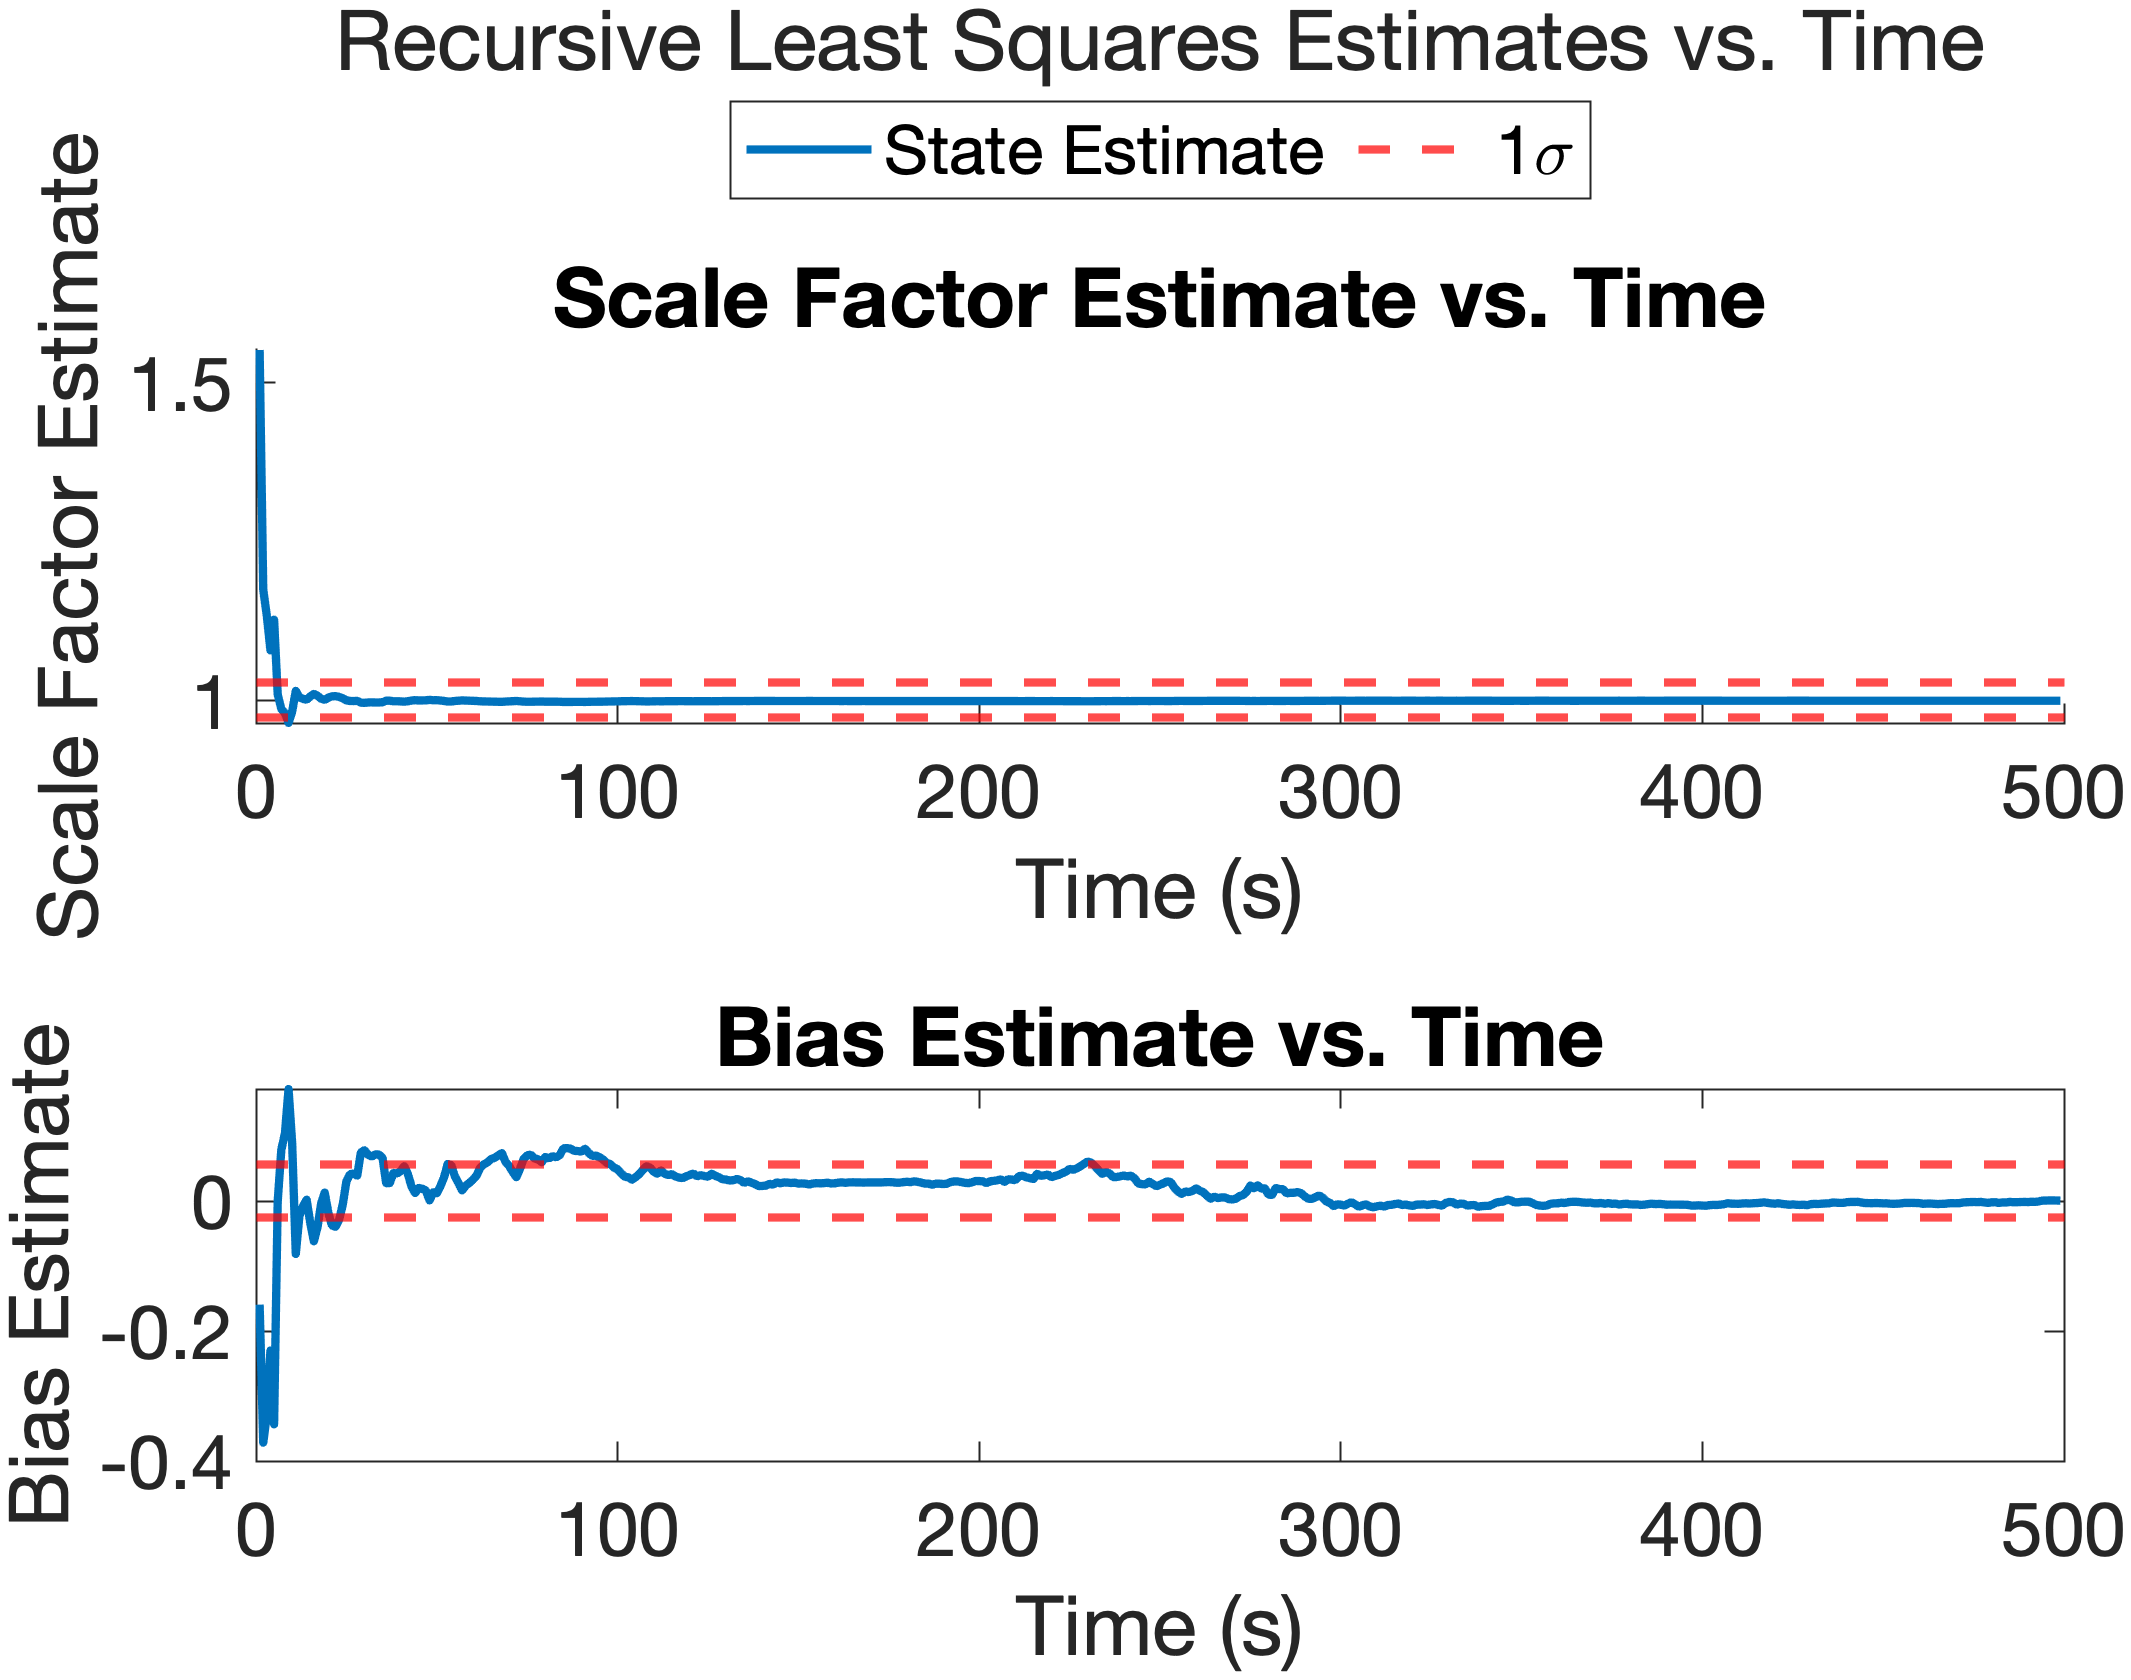
\includegraphics[width=0.75\linewidth]{../figures/p3d_state.png}\label{fig:p3d_state}
    \caption{State Estimates from Recursive Least Squares}
\end{figure}
\begin{figure}[H]
    \centering
    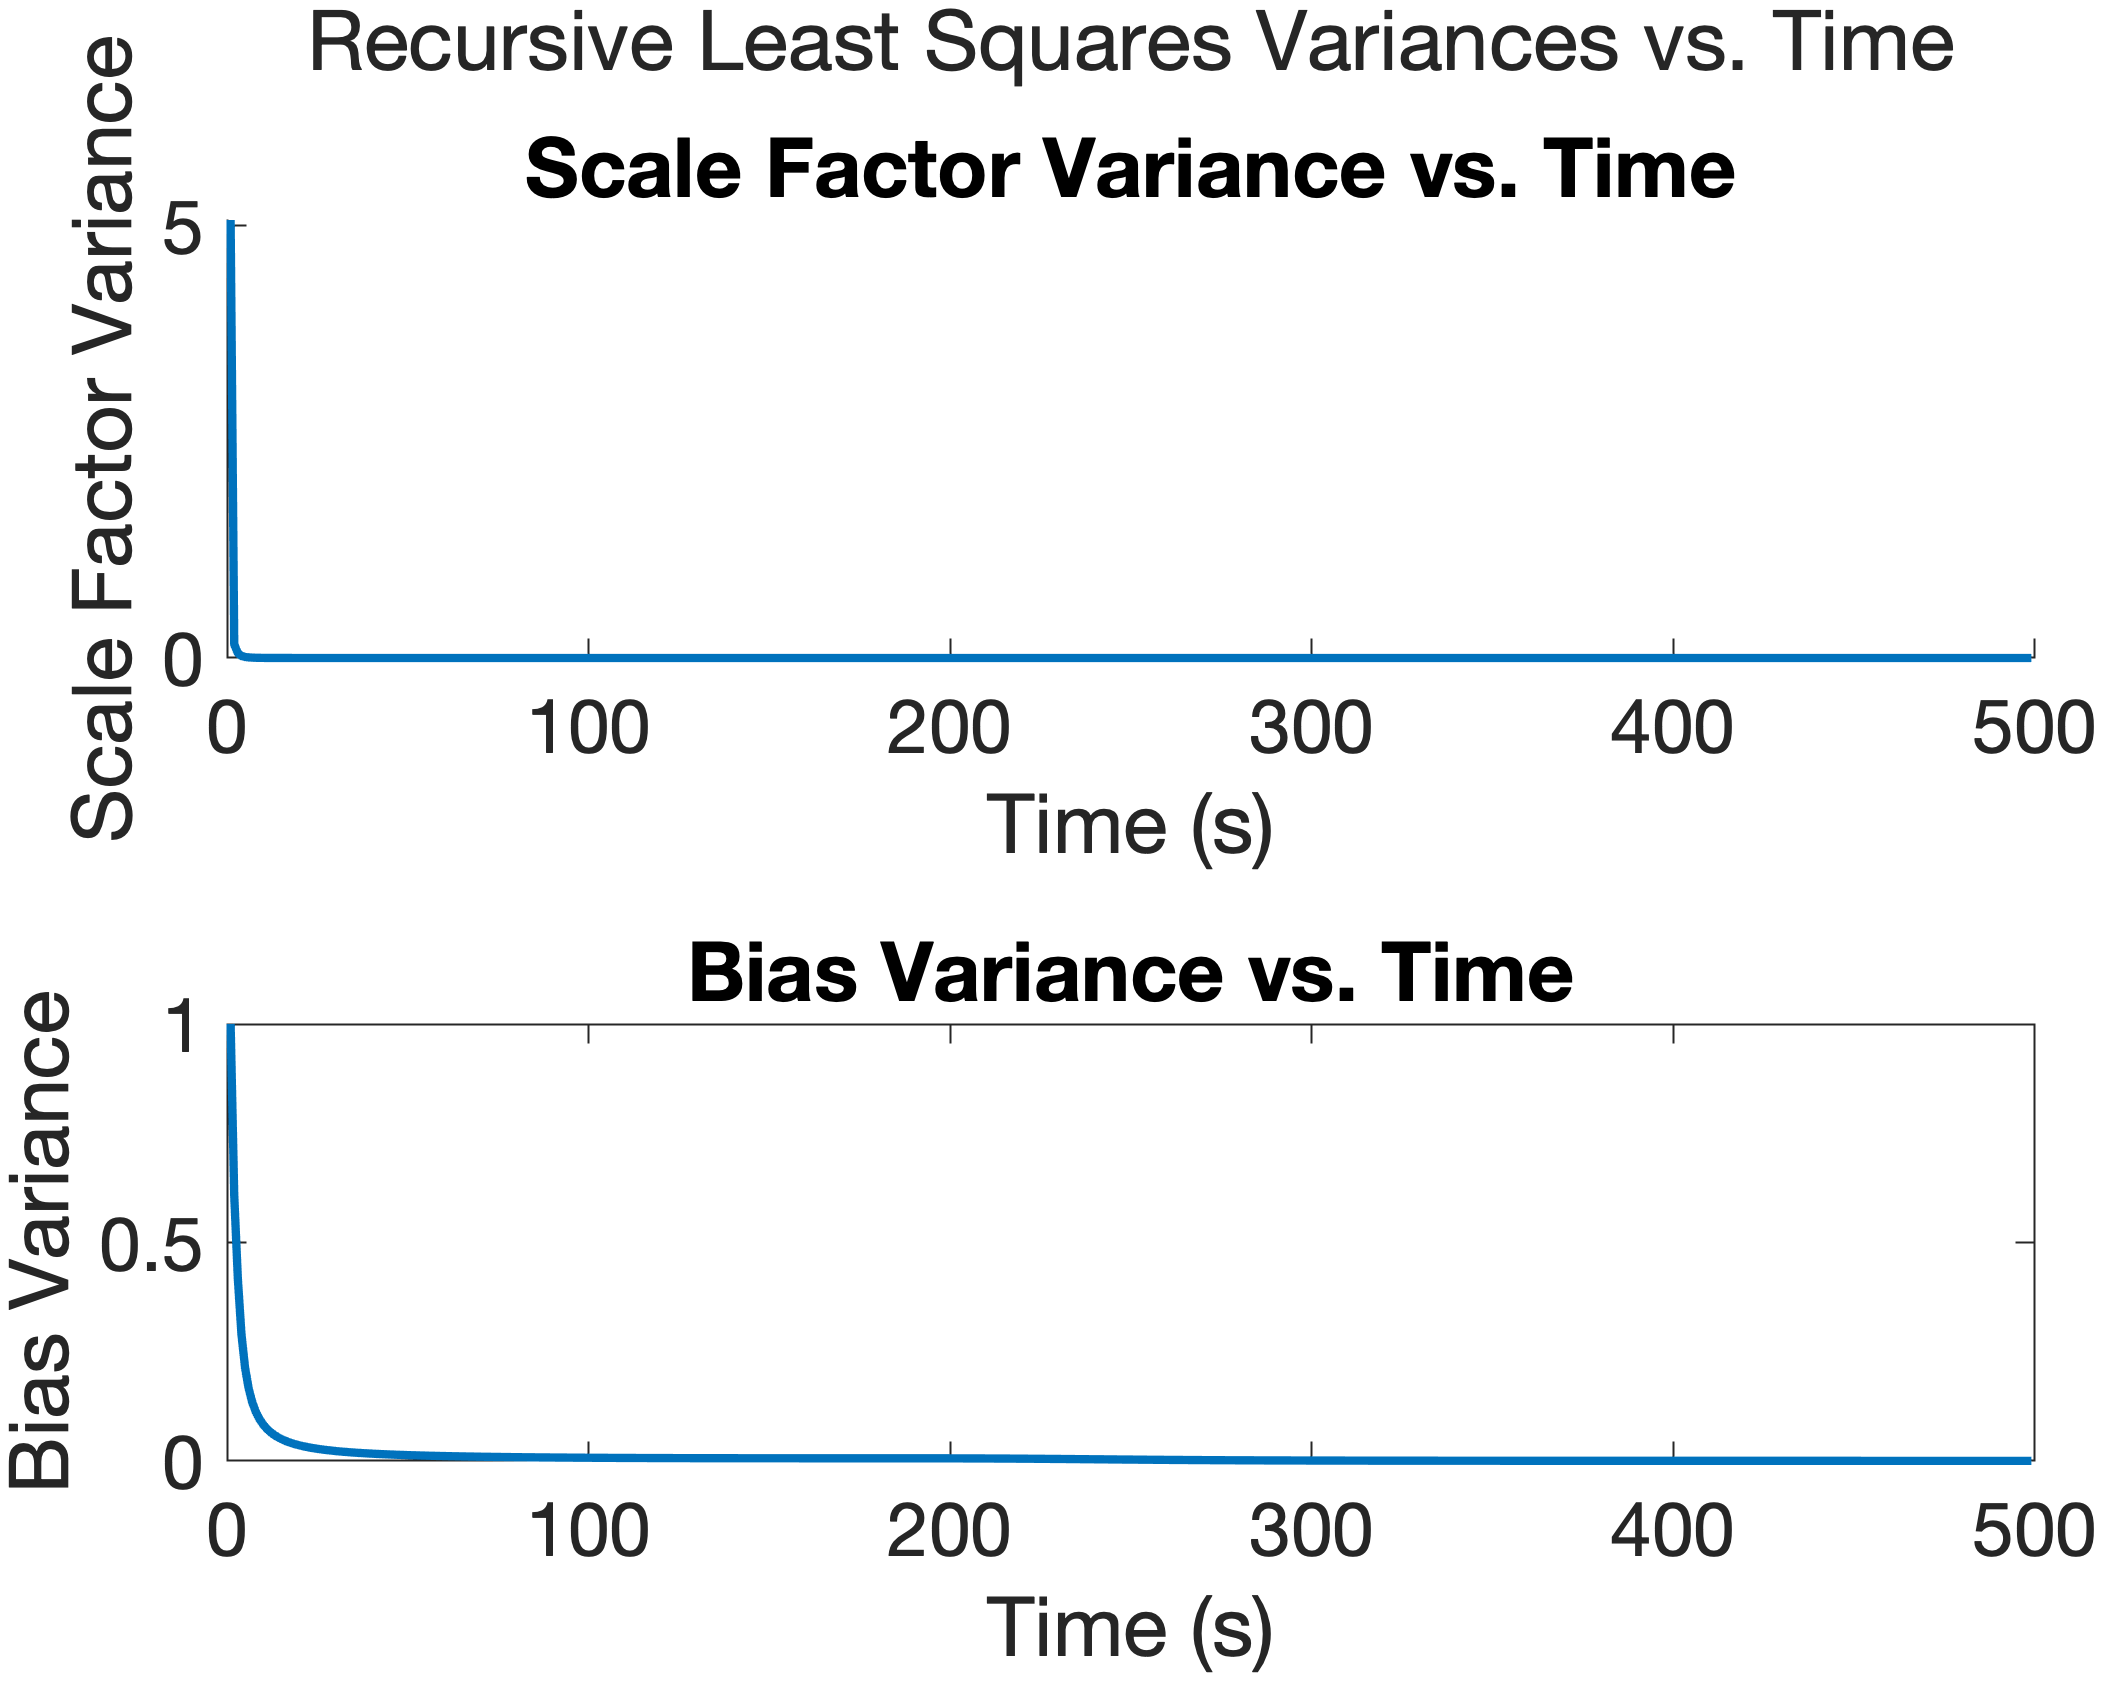
\includegraphics[width=0.75\linewidth]{../figures/p3d_variance.png}\label{fig:p3d_variance}
    \caption{State Estimates from Recursive Least Squares}
\end{figure}

\section*{Question IV}
Least Squares for System I.D. Simulate the following discrete system with a normal random input and output noise:
\begin{center}
    $G(z) = \frac{0.25(z - 0.8)}{z^2 - 1.90z + 0.95}$
\end{center}
\subsection*{Part A}
Develop the H matrix for the least squares solution.
\subsection*{Solution}
Before forming the H matrix and model of input to output given the coefficients of the transfer function is needed. This process is shown below:
\begin{gather*}
    G(z) = \frac{b_0 z - b_1}{z^2 - a_1z + a_2} \\
    y(k) + a_1 y(k-1) + a_2 y(k-2) = b_0 u(k-1) + b_1 u(k-2) \\
    y(k) = -a_1 y(k-1) - a_2 y(k-2) + b_0 u(k-1) + b_1 u(k-2) \\
    y(k+2) = -a_1 y(k+1) - a_2 y(k) + b_0 u(k+1) + b_1 u(k) \\
    H = \begin{bmatrix} -y(k+1) && -y(k) && u(k+1) && u(k) \end{bmatrix}
\end{gather*}

\subsection*{Part B}
Use least squares to estimate the coefficients of the above Transfer Function.  How good is the fit? Plot the bode response of the I.D. TF 
and the simulated TF on the same plot.  How much relative noise has been added (SNR - signal to noise ratio), plot $y$ and $Y$ on the same plot.
\subsection*{Solution}
\begin{figure}[H]
    \centering
    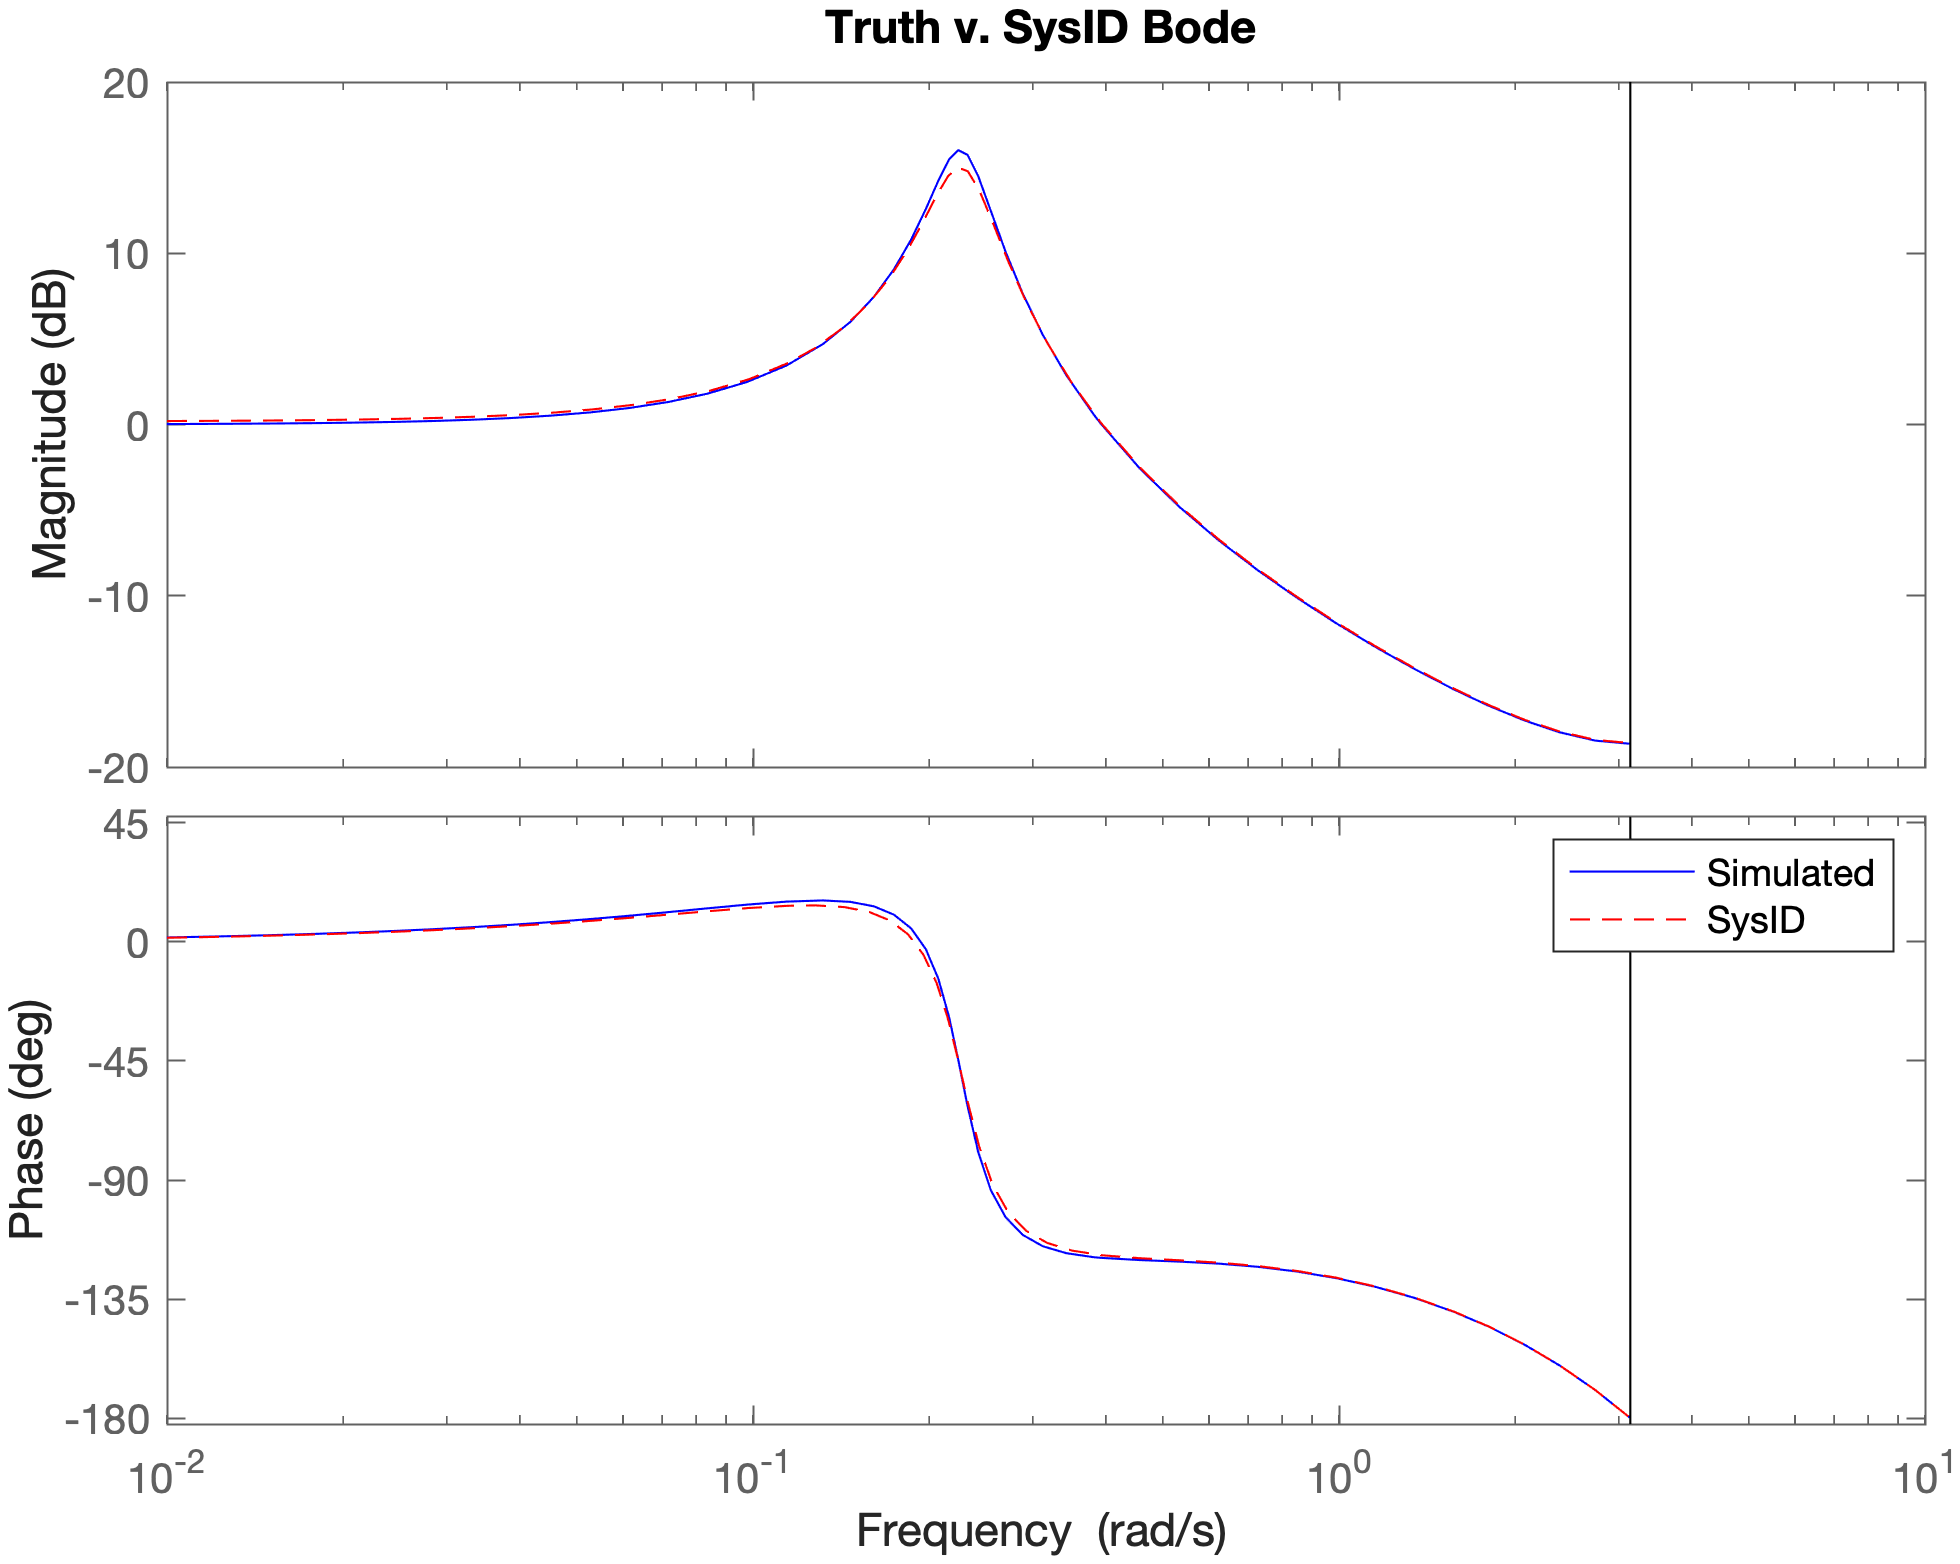
\includegraphics[width=0.75\linewidth]{../figures/p4b_bode.png}\label{fig:p4b_bode}
    \caption{Bode Plot of True TF \& SysID TF w/ $\sigma=0.01$}
\end{figure}
\begin{figure}[H]
    \centering
    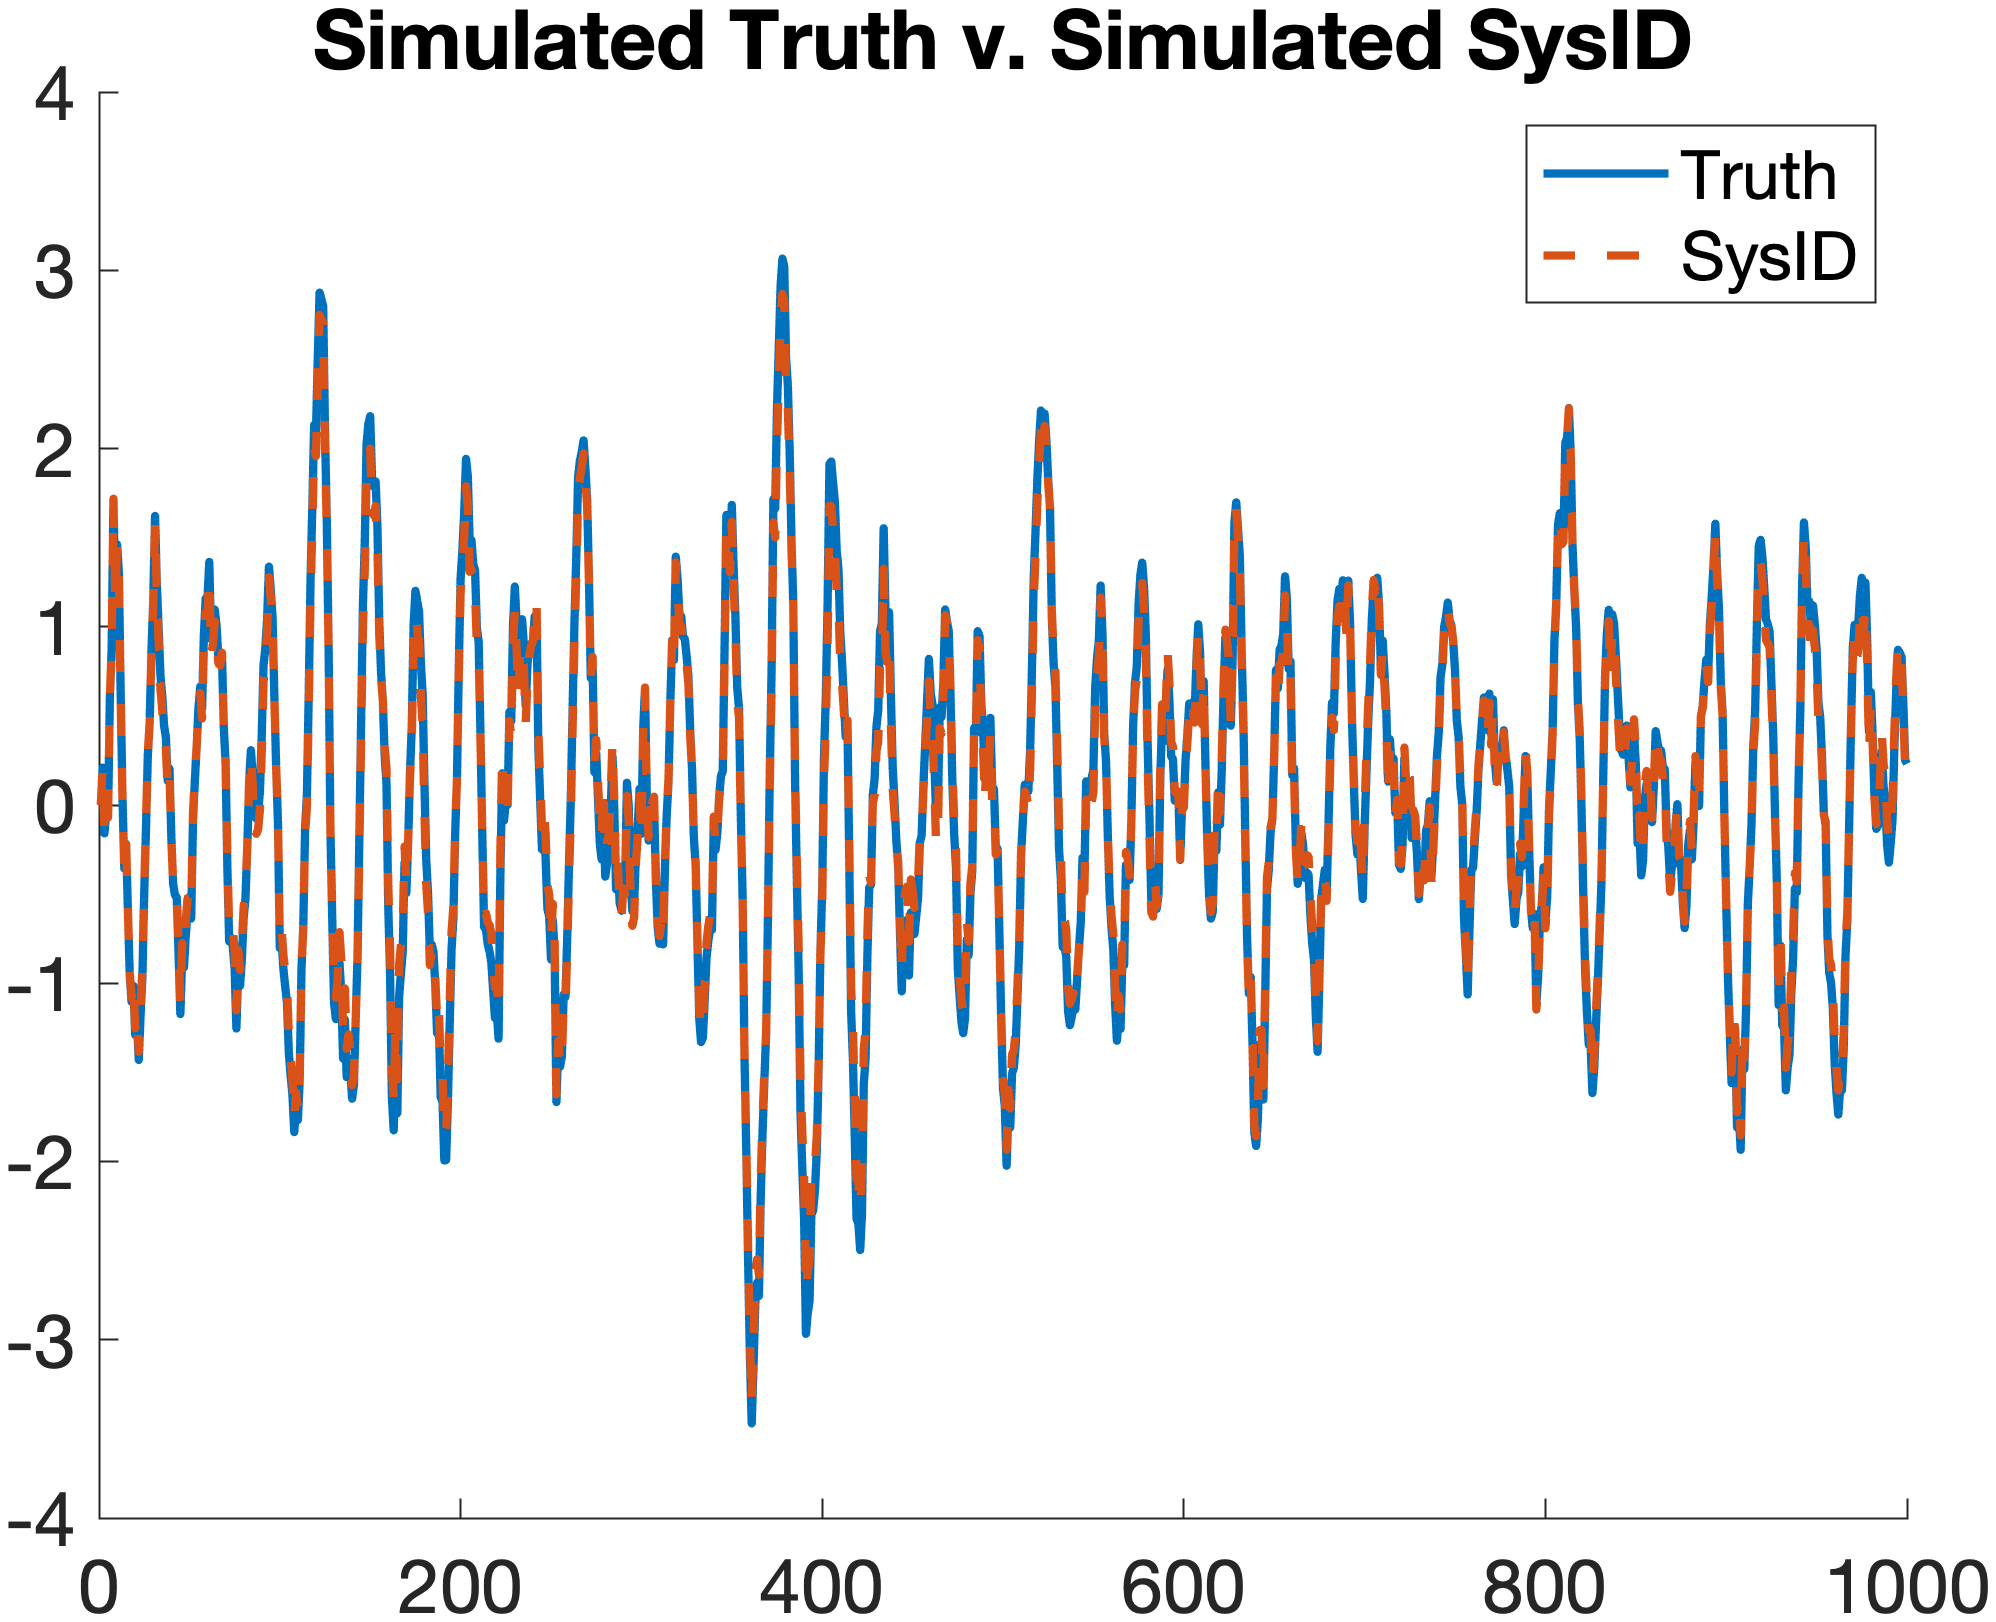
\includegraphics[width=0.75\linewidth]{../figures/p4b_tf.png}\label{fig:p4b_tf}
    \caption{Plot of True TF \& SysID TF w/ $\sigma=0.01$}
\end{figure}
The fit of the data is fairly close.  It can be seen that the system identification model is a good approximation of the real system. The SNR value 
for the system is 40.1726.  This is good as the signal is much stronger than the noise of the system.

\subsection*{Part C}
Repeat the estimation process about 10 times using new values for the noise vector each time.  Compute the mean and standard deviation of your 
parameter estimates.  Compare the computed values of the parameter statistics with those predicted by the theory based on the known value of 
the noise statistics.
\subsection*{Solution}
The 10-run Monte Carlo Simulation yields a mean $\bar{x} = \begin{bmatrix} -1.8922 \\ 0.9426 \\ 0.2497 \\ -0.1976 \end{bmatrix}$ and standard deviation 
$\sigma = \begin{bmatrix} 0.0011 \\ 0.0011 \\ \sim 0 \\ \sim 0 \end{bmatrix}$.  The analytical equivalent mean is just the original parameters of transfer 
function.  The analytical and numerical means appear to match fairly well, of course with a small amount of deviation.  The analytical standard deviation 
is calculated as follows:
\begin{equation}
    \sigma = \sigma_n (H^T H)^{-1}
\end{equation}
This yields an analytical standard deviation of $\sigma = \begin{bmatrix} 0.0016 \\ 0.0016 \\ \sim 0 \\ \sim 0 \end{bmatrix}$.  This is very nearly the same 
as the numerical solution.

\subsection*{Part D}
Now use sigma between 0.1 and 1.0 and repeat parts b and c.
\subsection*{Solution}
\begin{figure}[H]
    \centering
    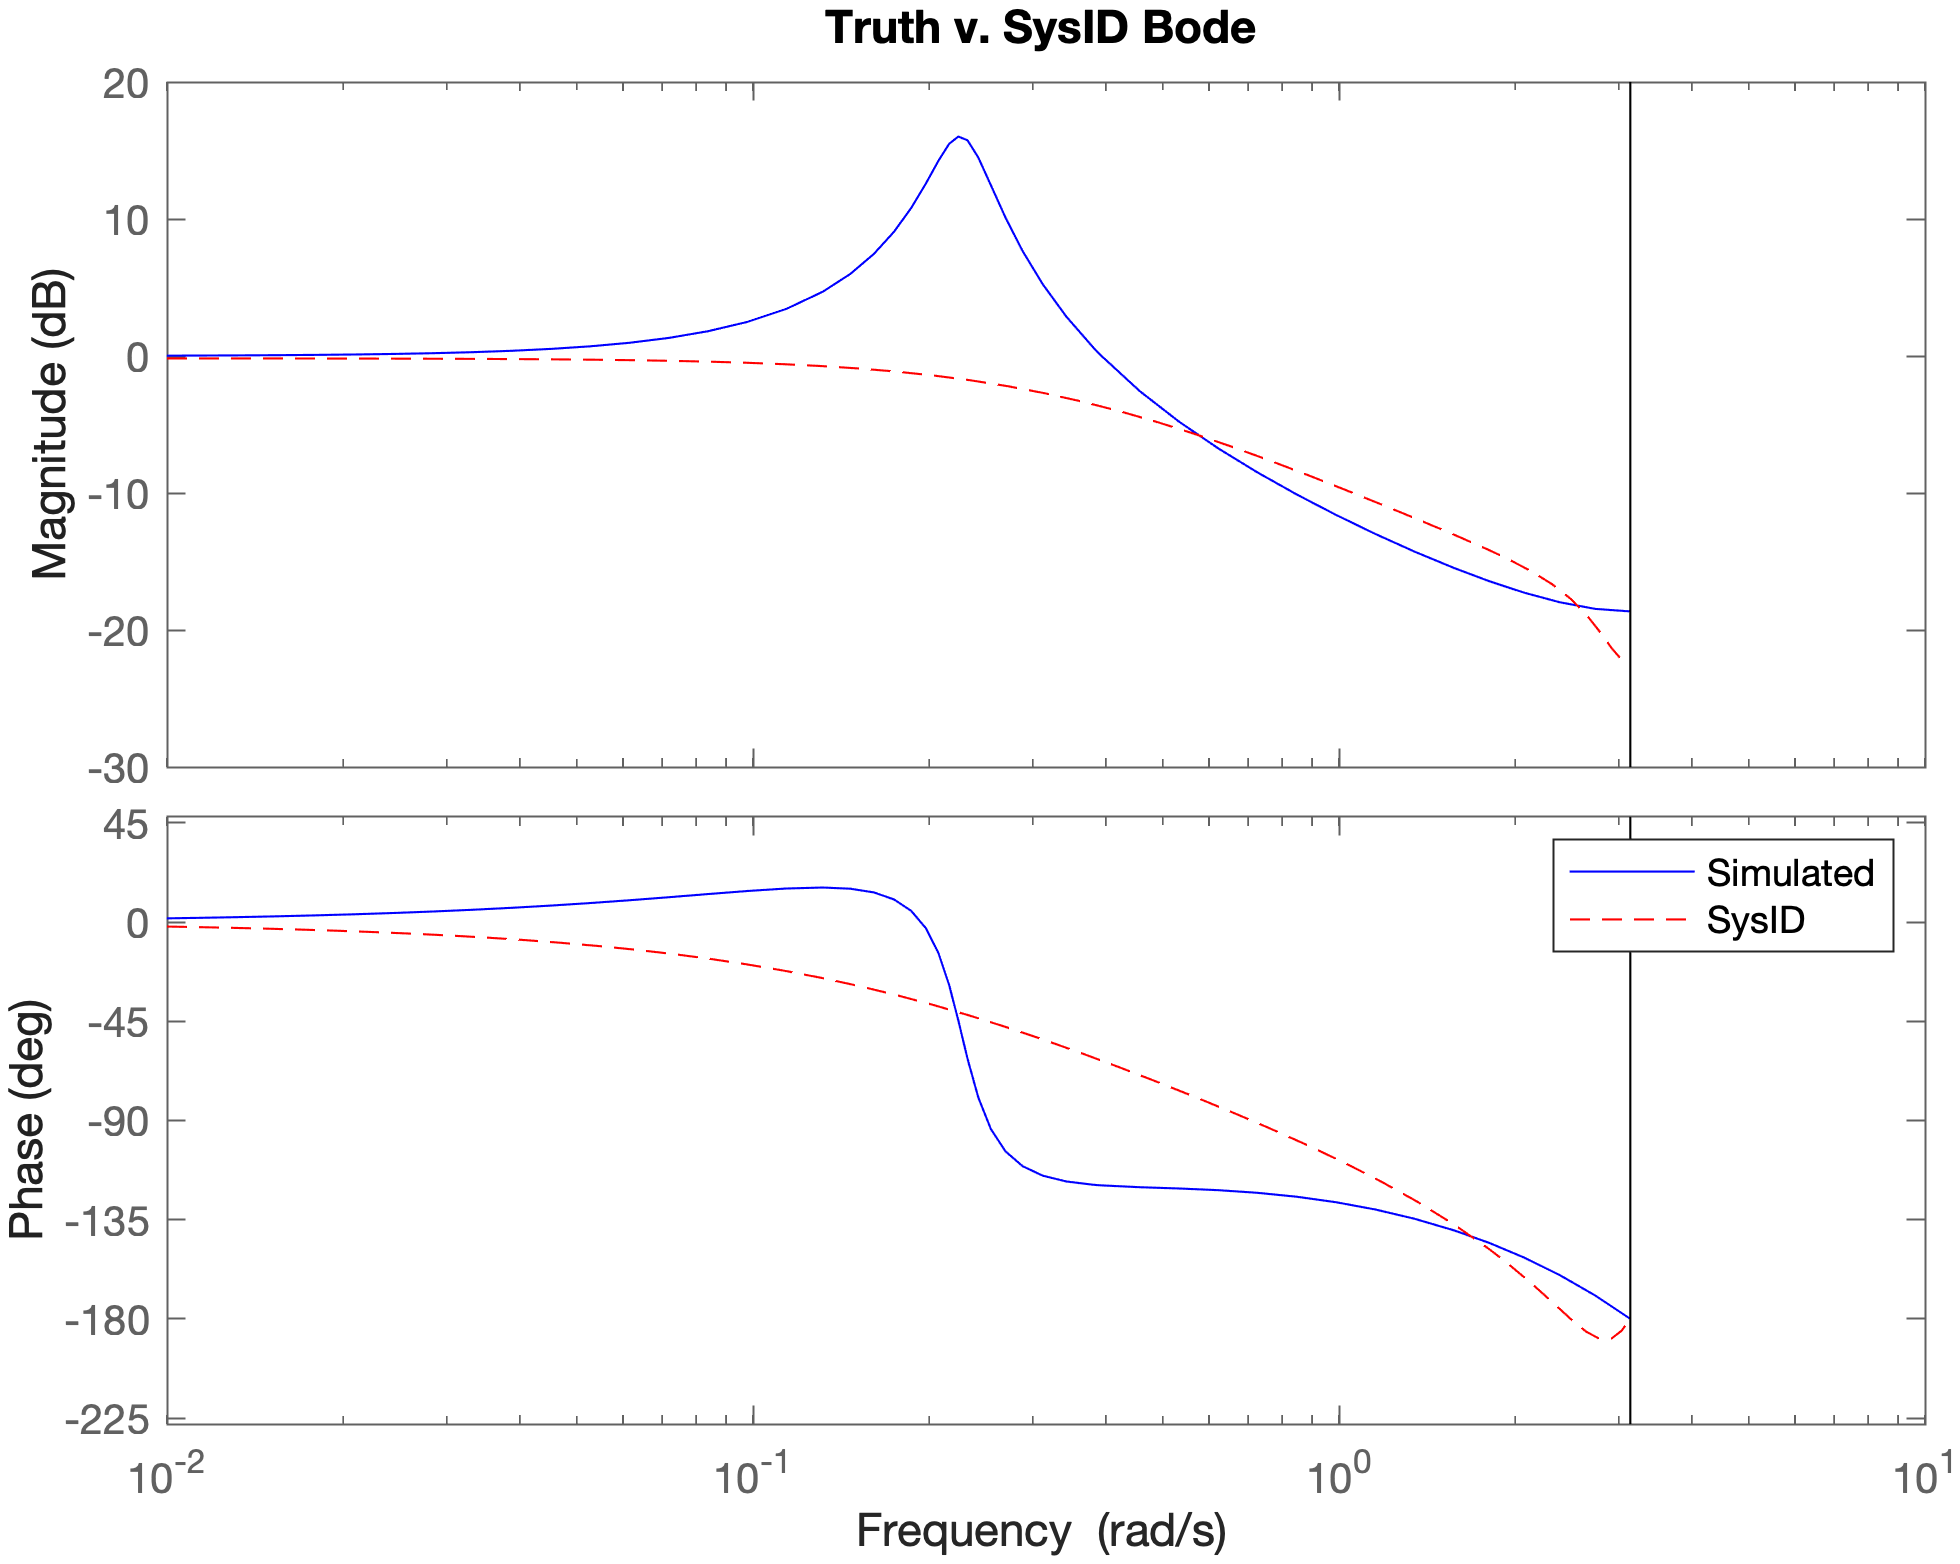
\includegraphics[width=0.75\linewidth]{../figures/p4d_bode.png}\label{fig:p4d_bode}
    \caption{Bode Plot of True TF \& SysID TF w/ $\sigma=0.9$}
\end{figure}
\begin{figure}[H]
    \centering
    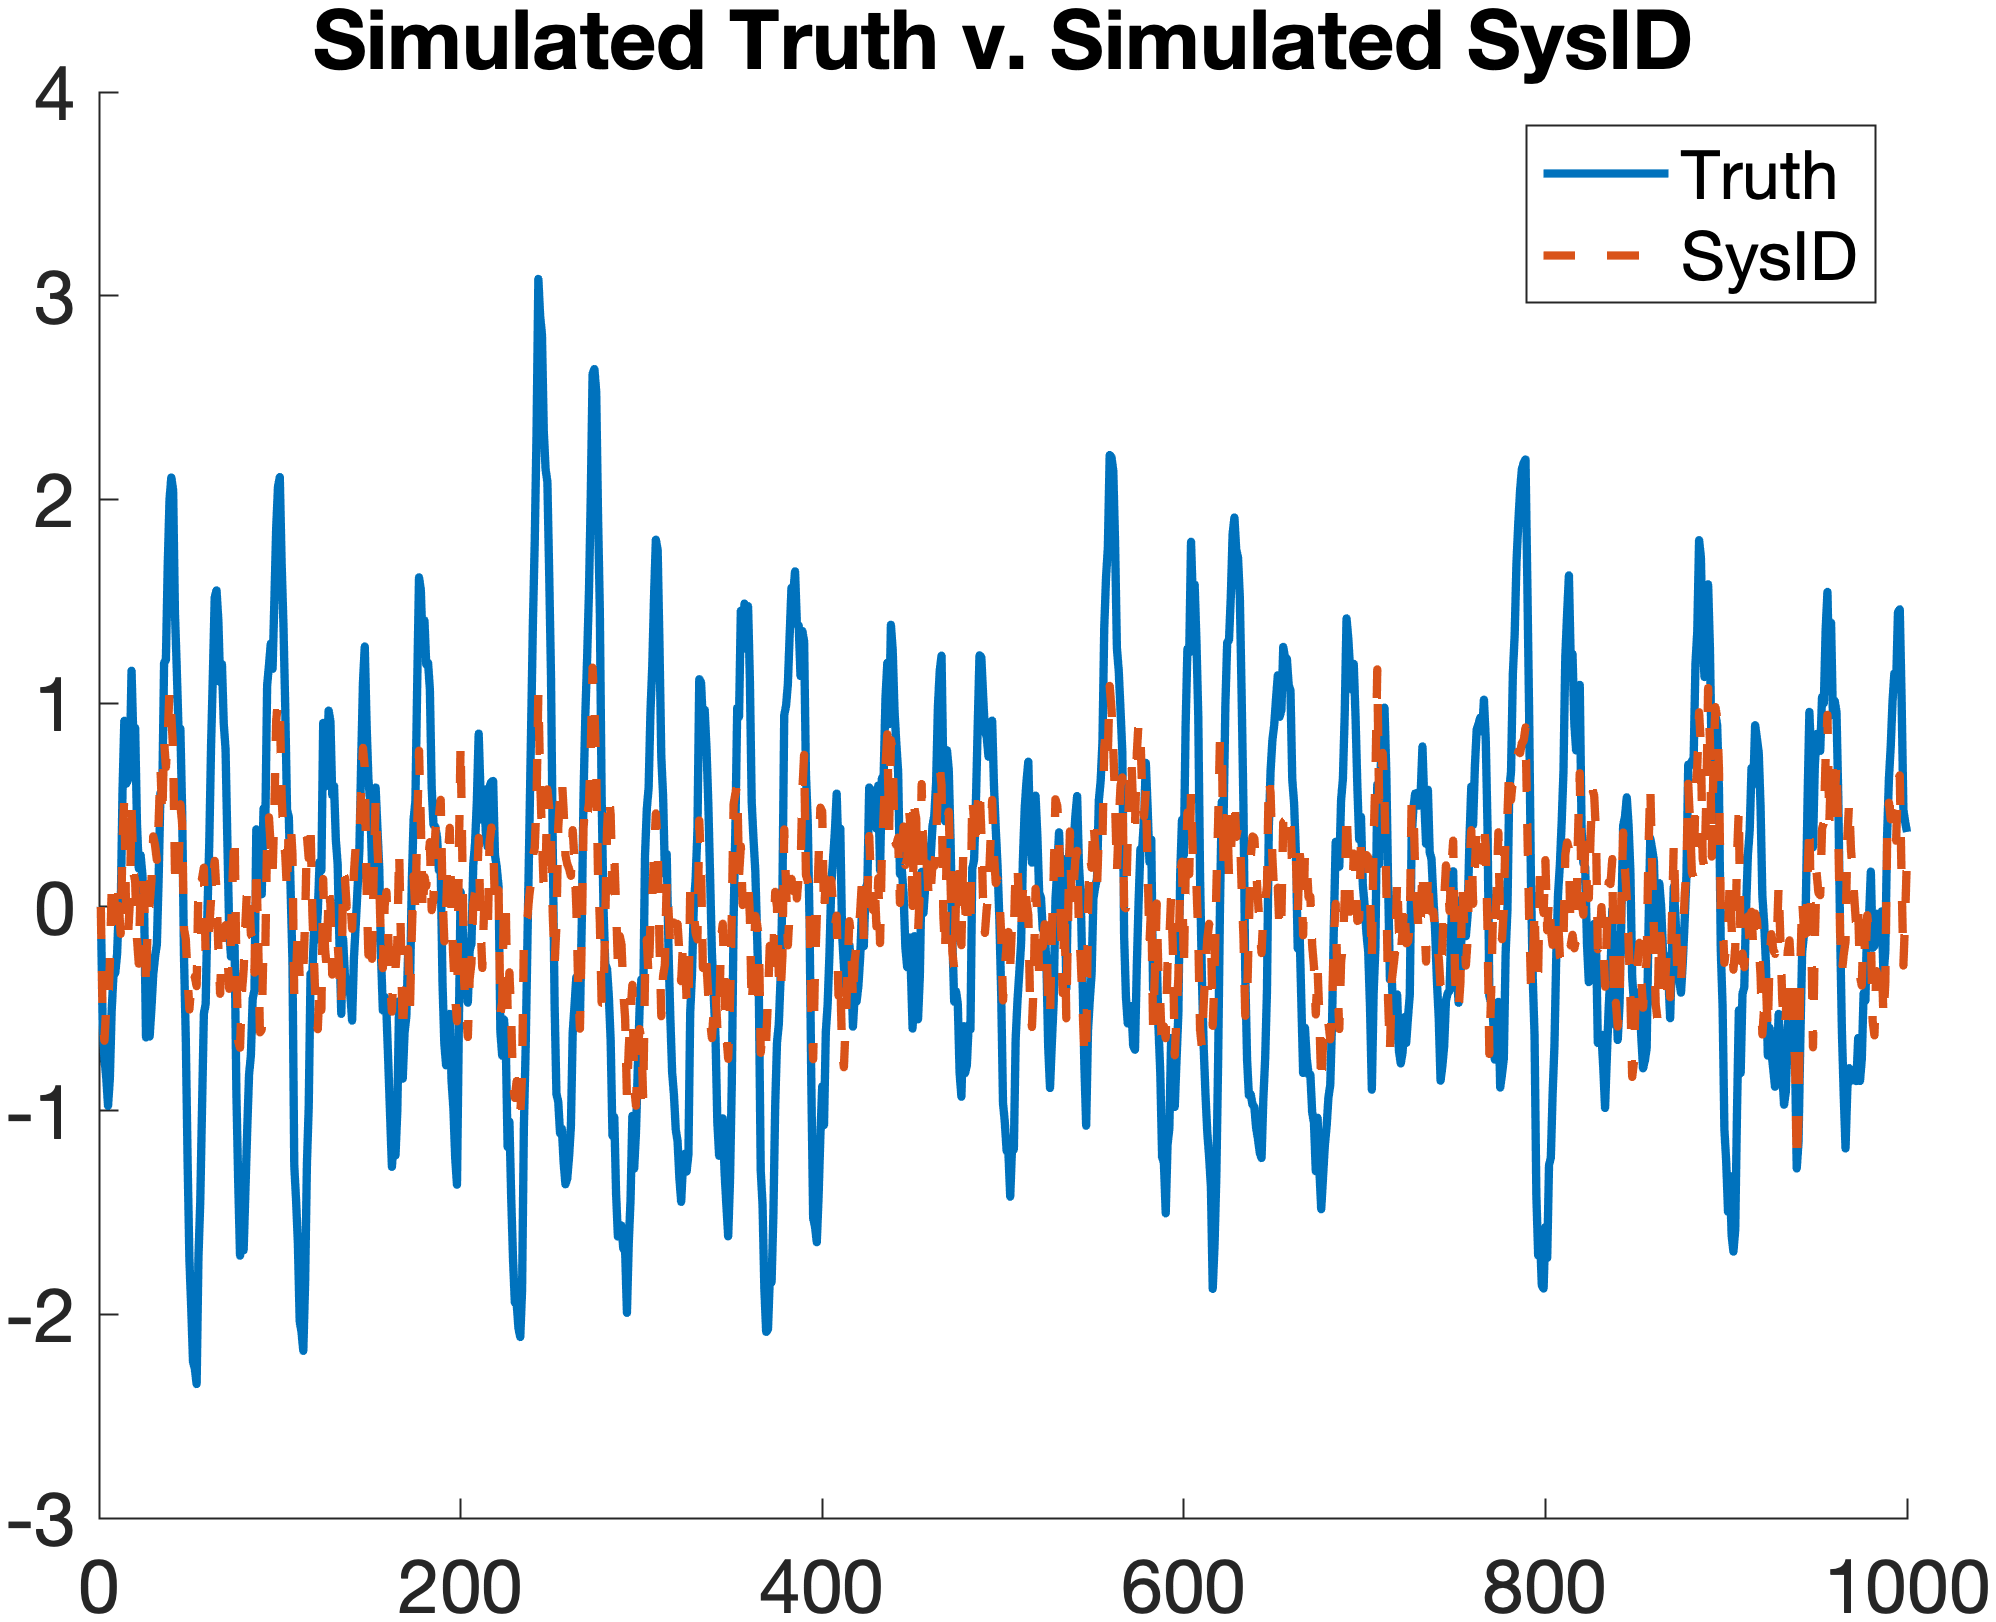
\includegraphics[width=0.75\linewidth]{../figures/p4d_tf.png}\label{fig:p4d_tf}
    \caption{Plot of True TF \& SysID TF w/ $\sigma=0.9$}
\end{figure}
The fit is nowhere near as good as in Part B. Truly, it isn't even a valid representation of the system at this point.  The SNR for this scenario 
is 1.3027 meaning the noise is a lot more prevalent in this case. \\
The Monte Carlo, utilizing the new $\sigma$ value of 0.9, yields a numerical mean of $\bar{x} = \begin{bmatrix} -0.3208 \\ -0.2968 \\ 0.2659 \\ 0.1790 \end{bmatrix}$
which is not close to the original transfer function coefficients.  The numerical $\sigma$ for this scenario is 
$\sigma = \begin{bmatrix} 0.0291 \\ 0.0209 \\ 0.0358 \\ 0.0285 \end{bmatrix}$.  The analytical $\sigma$ for the same scenario is 
$\sigma = \begin{bmatrix} 0.0260 \\ 0.0255 \\ 0.0287 \\ 0.0294 \end{bmatrix}$.  While this does match the numerical solution's $\sigma$ rather closely, the 
more important observation is that increasing the $\sigma$ on the noise greatly increases the $\sigma$ on the solution.

\subsection*{Part E}
What can you conclude about using least squares for sys id with large amounts of noise?
\subsection*{Solution}
Least Squares for system identification is good for low SNR systems, but it breaks down rather quickly with high SNR systems.

\section*{Question V}
Justification of white noise for certain problems. Consider two problems: (i) Simple first order low-pass filter with bandlimited white noise as the input:\\
$y = G(s)\omega$, so that $S_y(j\omega) = |G(j\omega)|^2 S_w(j\omega)$, and the noise has the PSD:
\begin{gather*}
    S_1(\omega) = \left\{
                    \begin{array}{lr}
                        A, & |\omega|\leq\omega_c\\
                        0, & |\omega|>\omega_c
                    \end{array}
                \right\}\\
    G(s)=\frac{1}{T_ws+1}
\end{gather*}
(ii) The same low pass system, but with pure white noise as the input.
\begin{gather*}
    S_2(\omega)=A,\forall\omega\\
    G(s)=\frac{1}{T_ws+1}
\end{gather*}
The first case seems quite plausible, but the second case has an input with infinite variance and so is not physically realizable.  However, the white noise 
assumption simplifies the system analysis significantly, so it is important to see if the assumption is justified.  We test this with our two examples above.
\subsection*{Part A}
Sketch the noise PSD and $|G(j\omega)|$ for a reasonable value of $T_w$ and $\omega_c$ to compare the two cases.
\subsection*{Solution}
\begin{figure}[H]
    \centering
    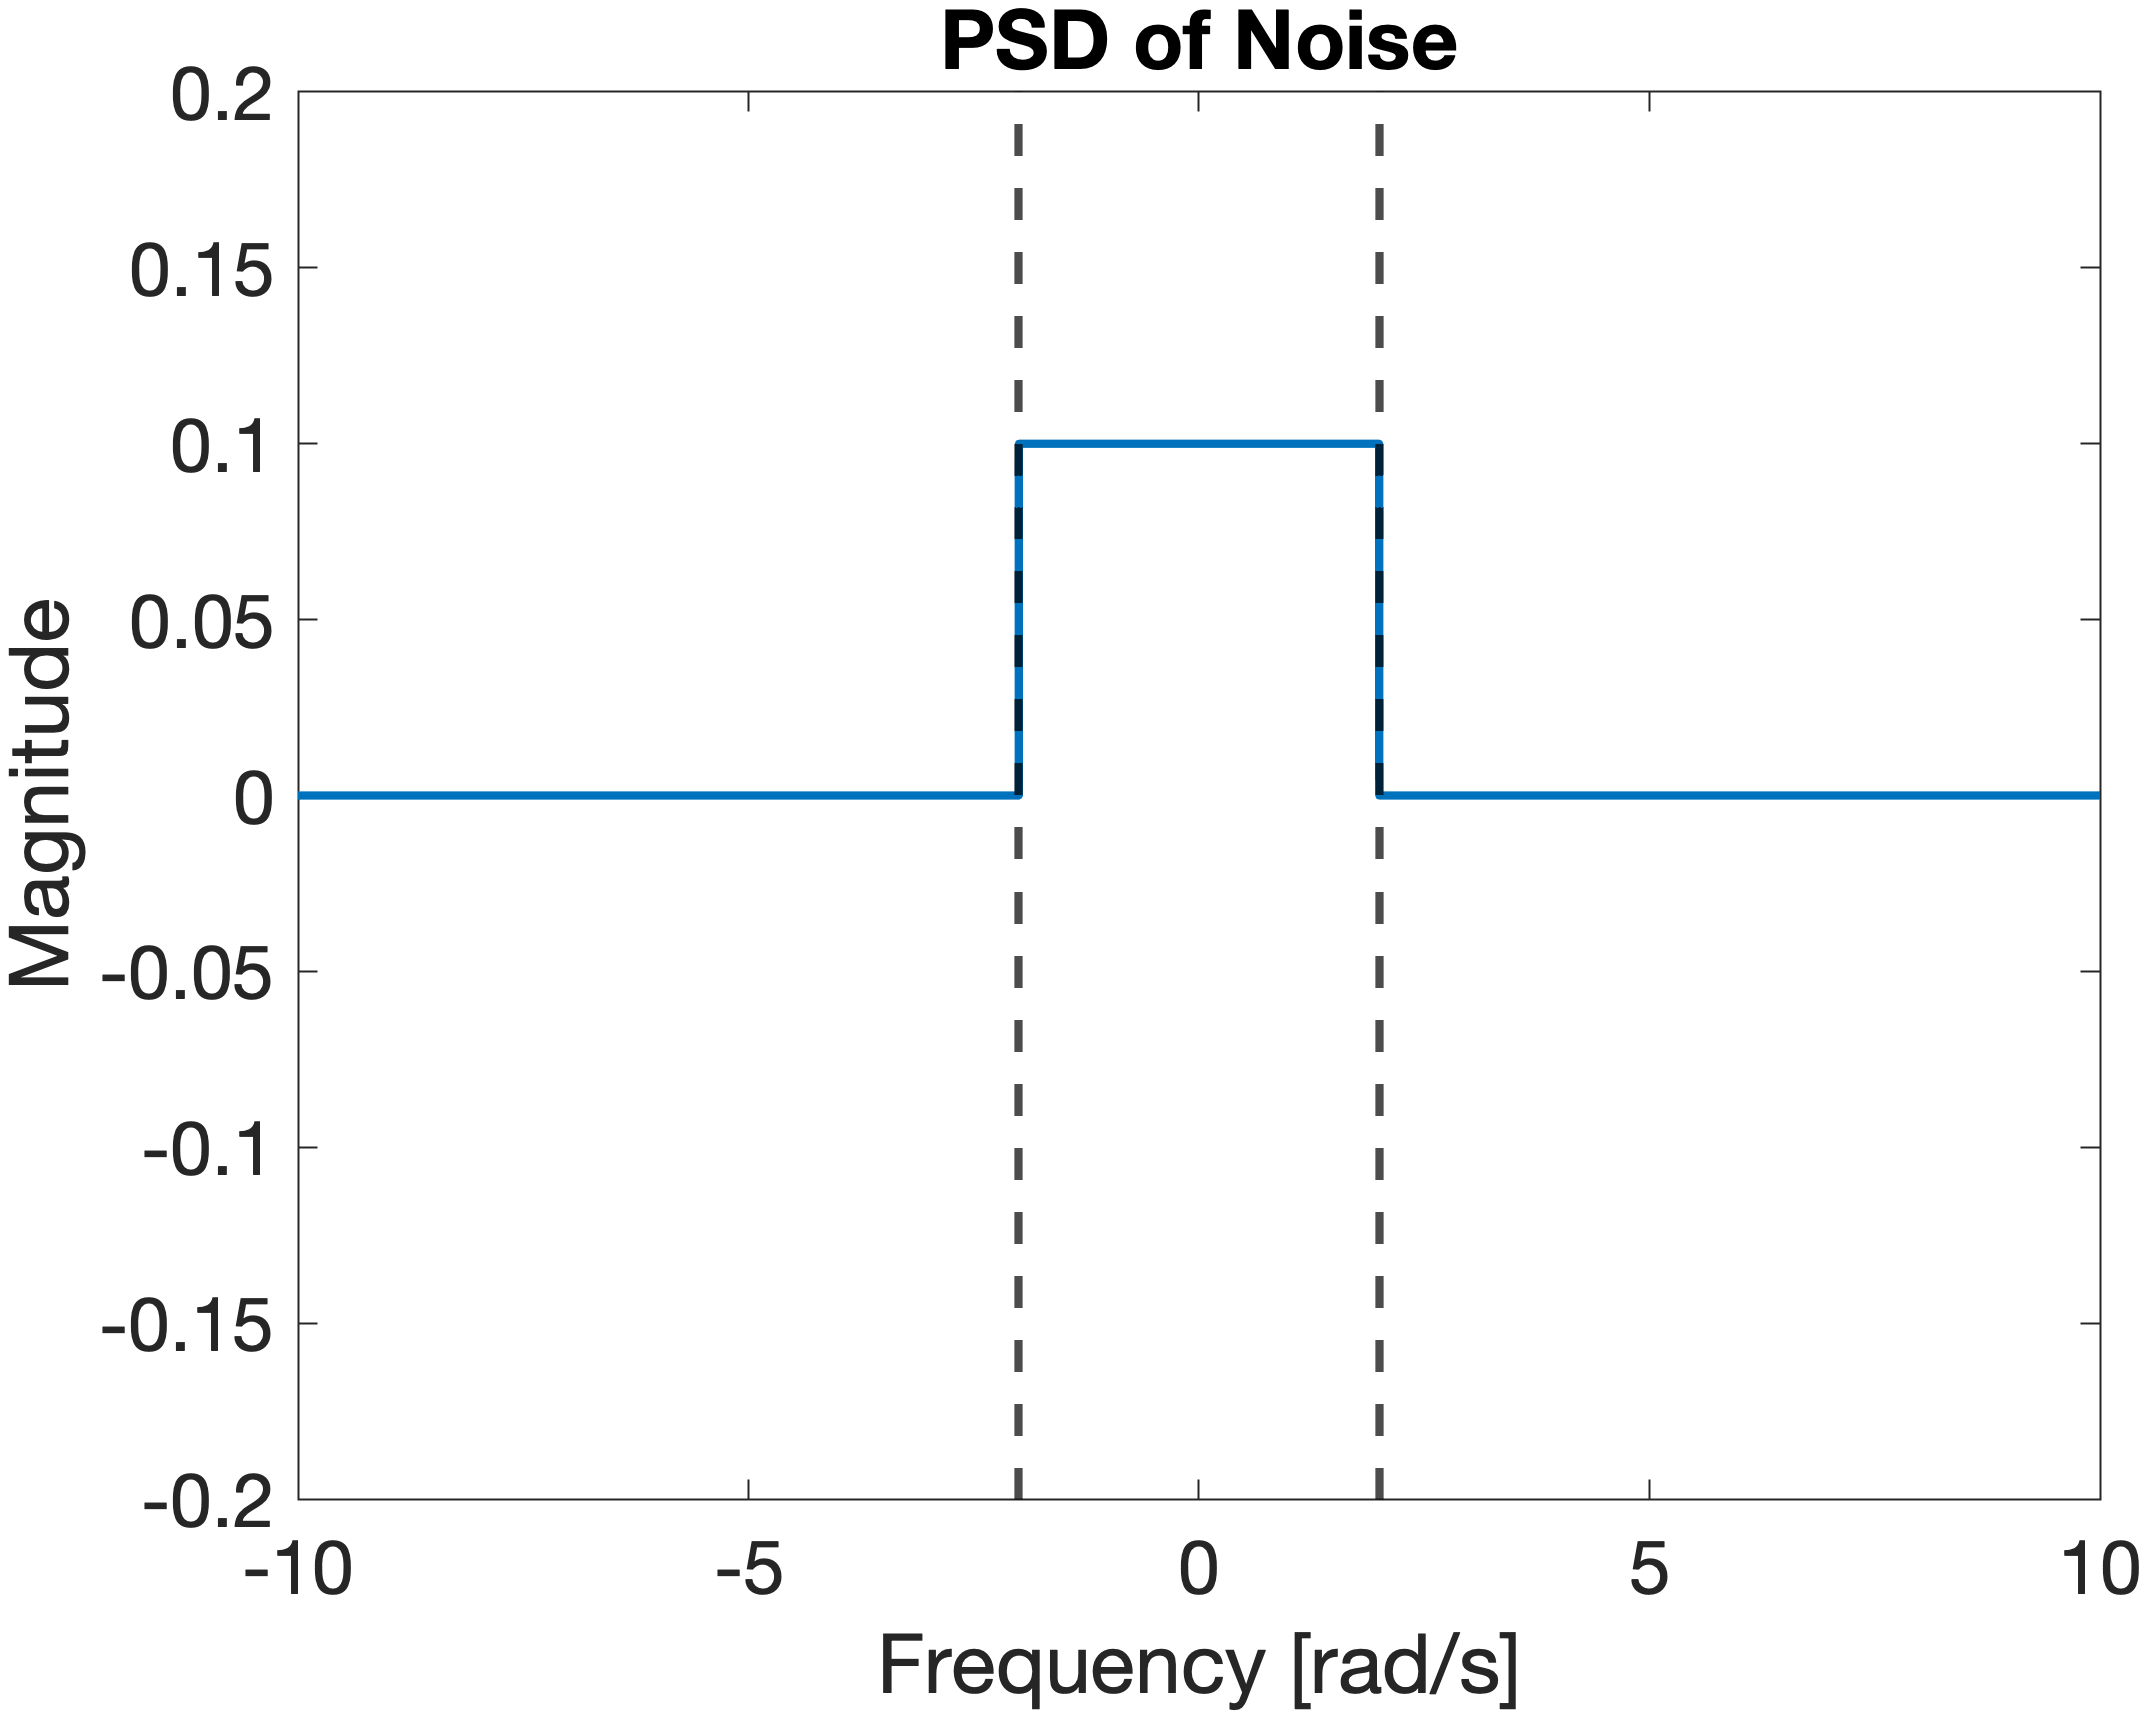
\includegraphics[width=0.75\linewidth]{../figures/p5_noise_psd.png}\label{fig:p5_noise_psd}
    \caption{Noise PSD}
\end{figure}
\begin{figure}[H]
    \centering
    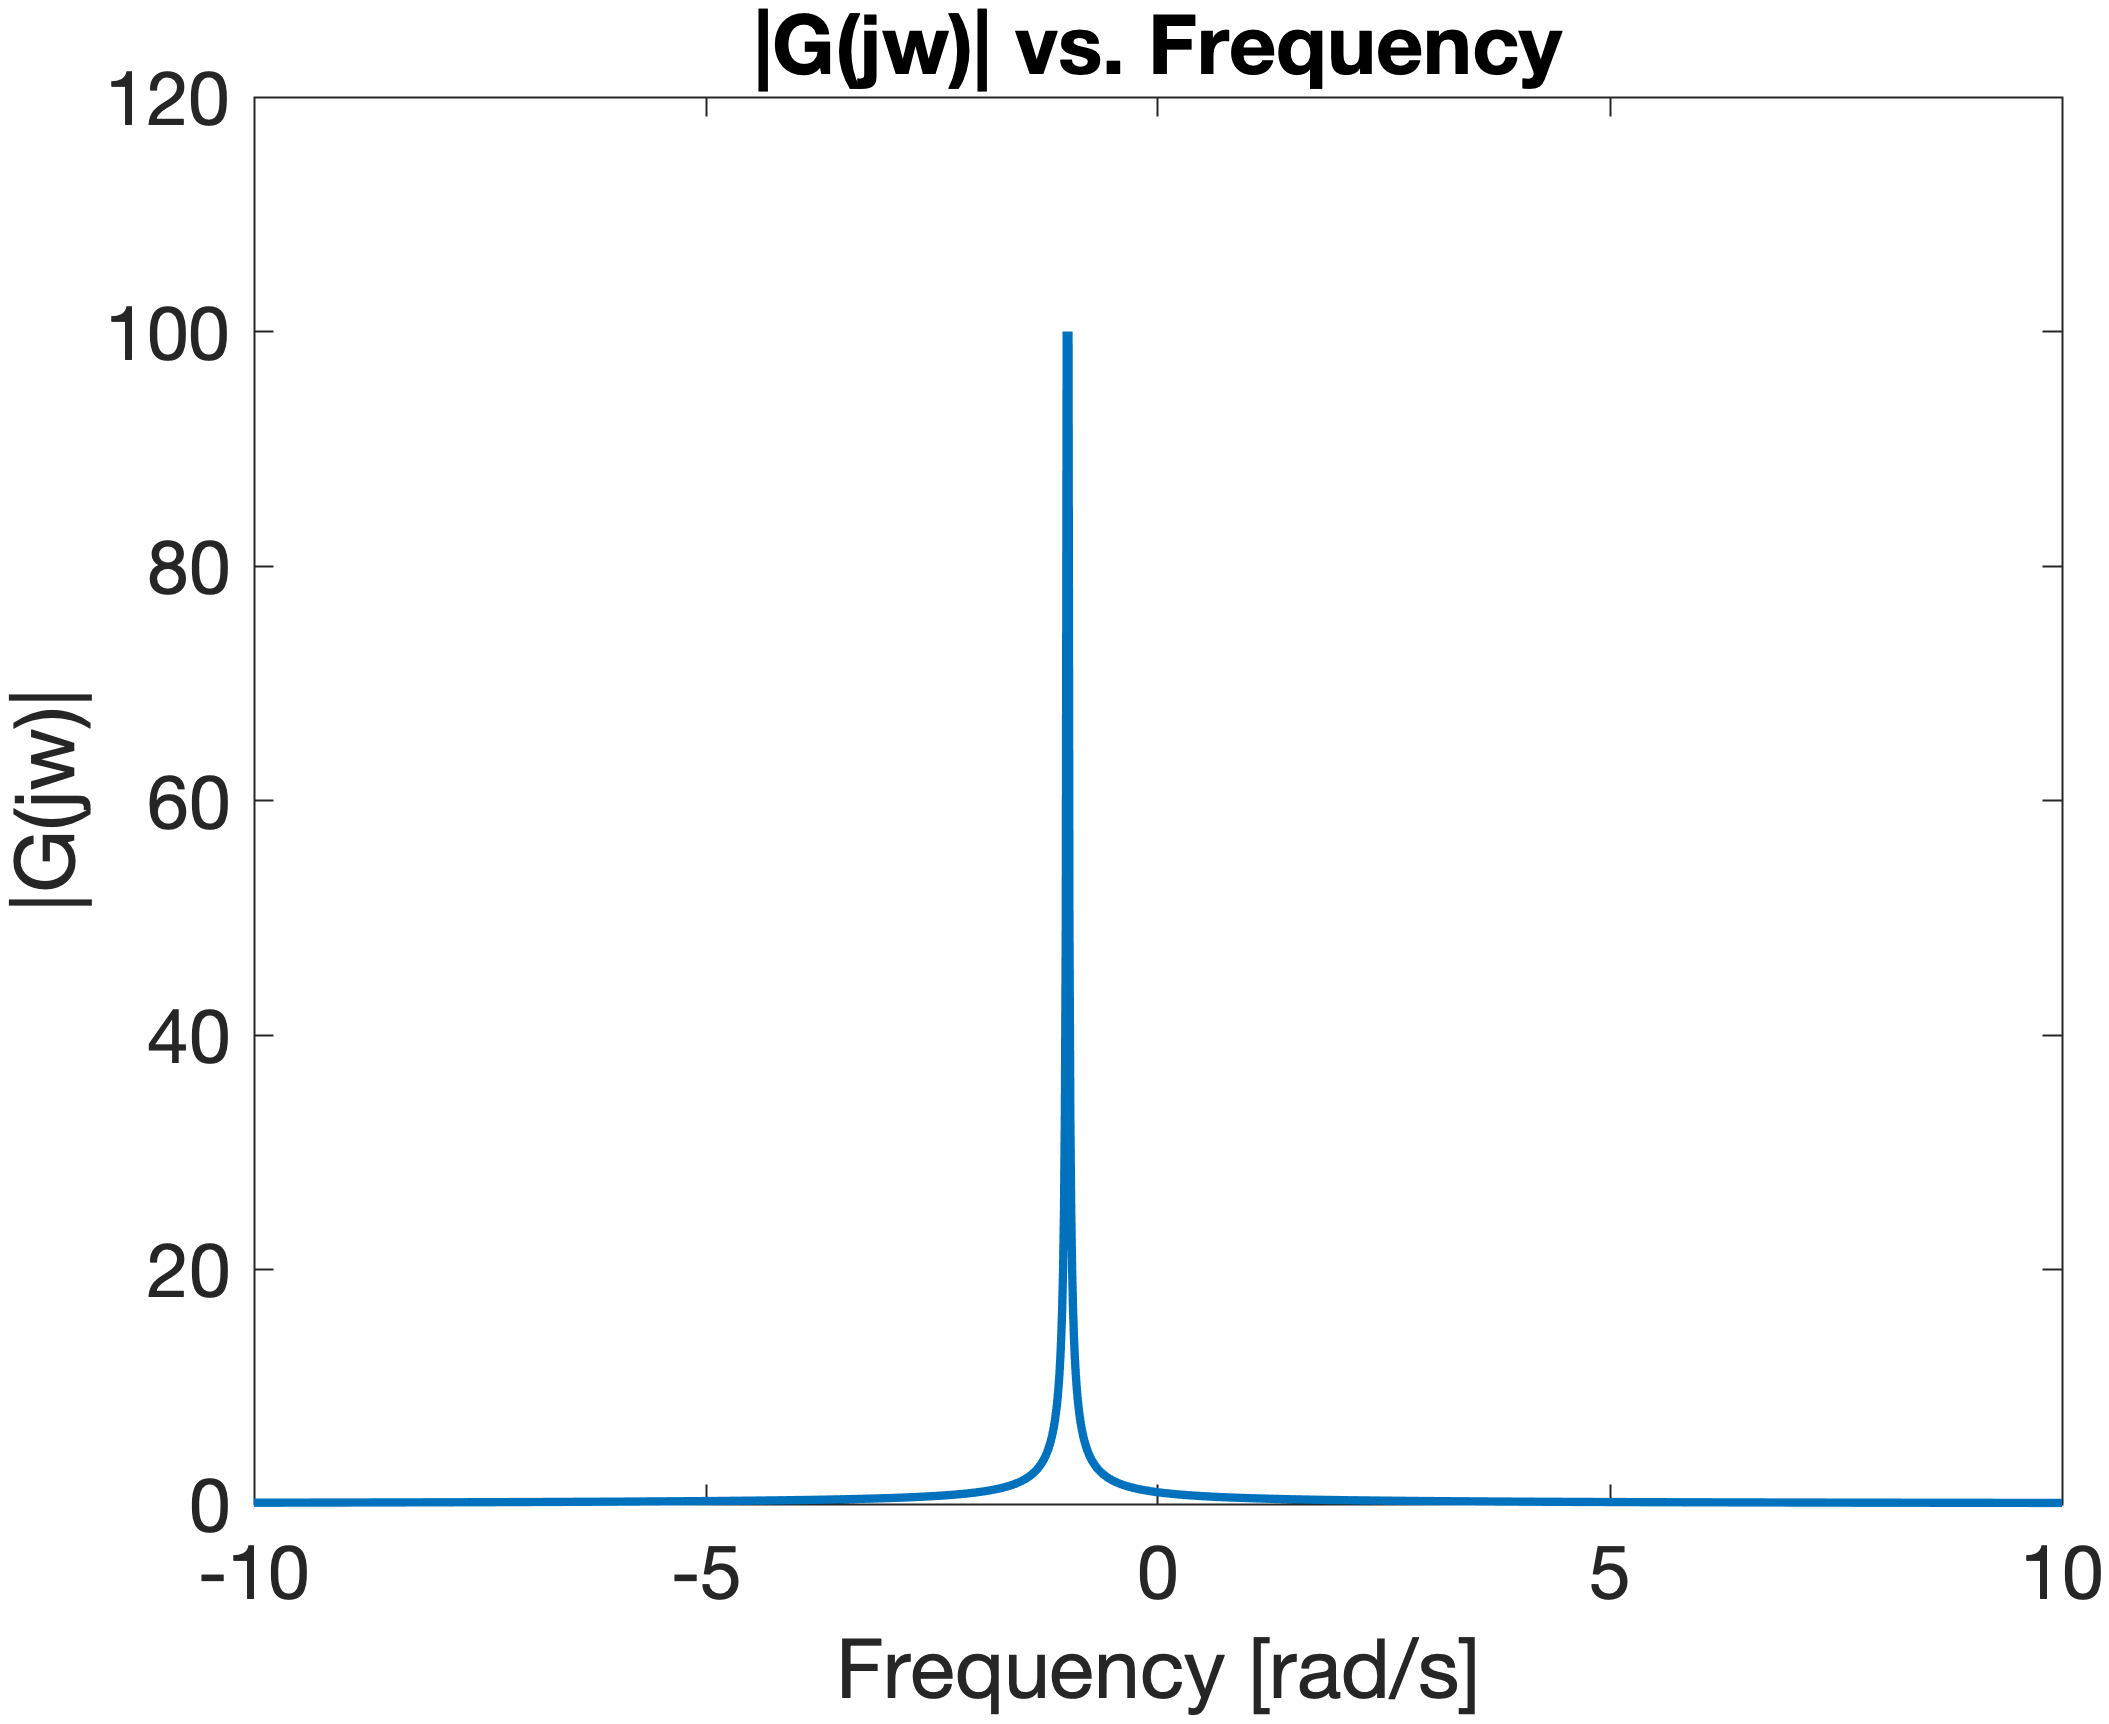
\includegraphics[width=0.75\linewidth]{../figures/p5_gjw.png}\label{fig:p5_gjw}
    \caption{$|G(j\omega)|$}
\end{figure}

\subsection*{Part B}
Determine the $S_y(j\omega)$ for the two cases.  Sketch these too.
\subsection*{Solution}
\begin{figure}[H]
    \centering
    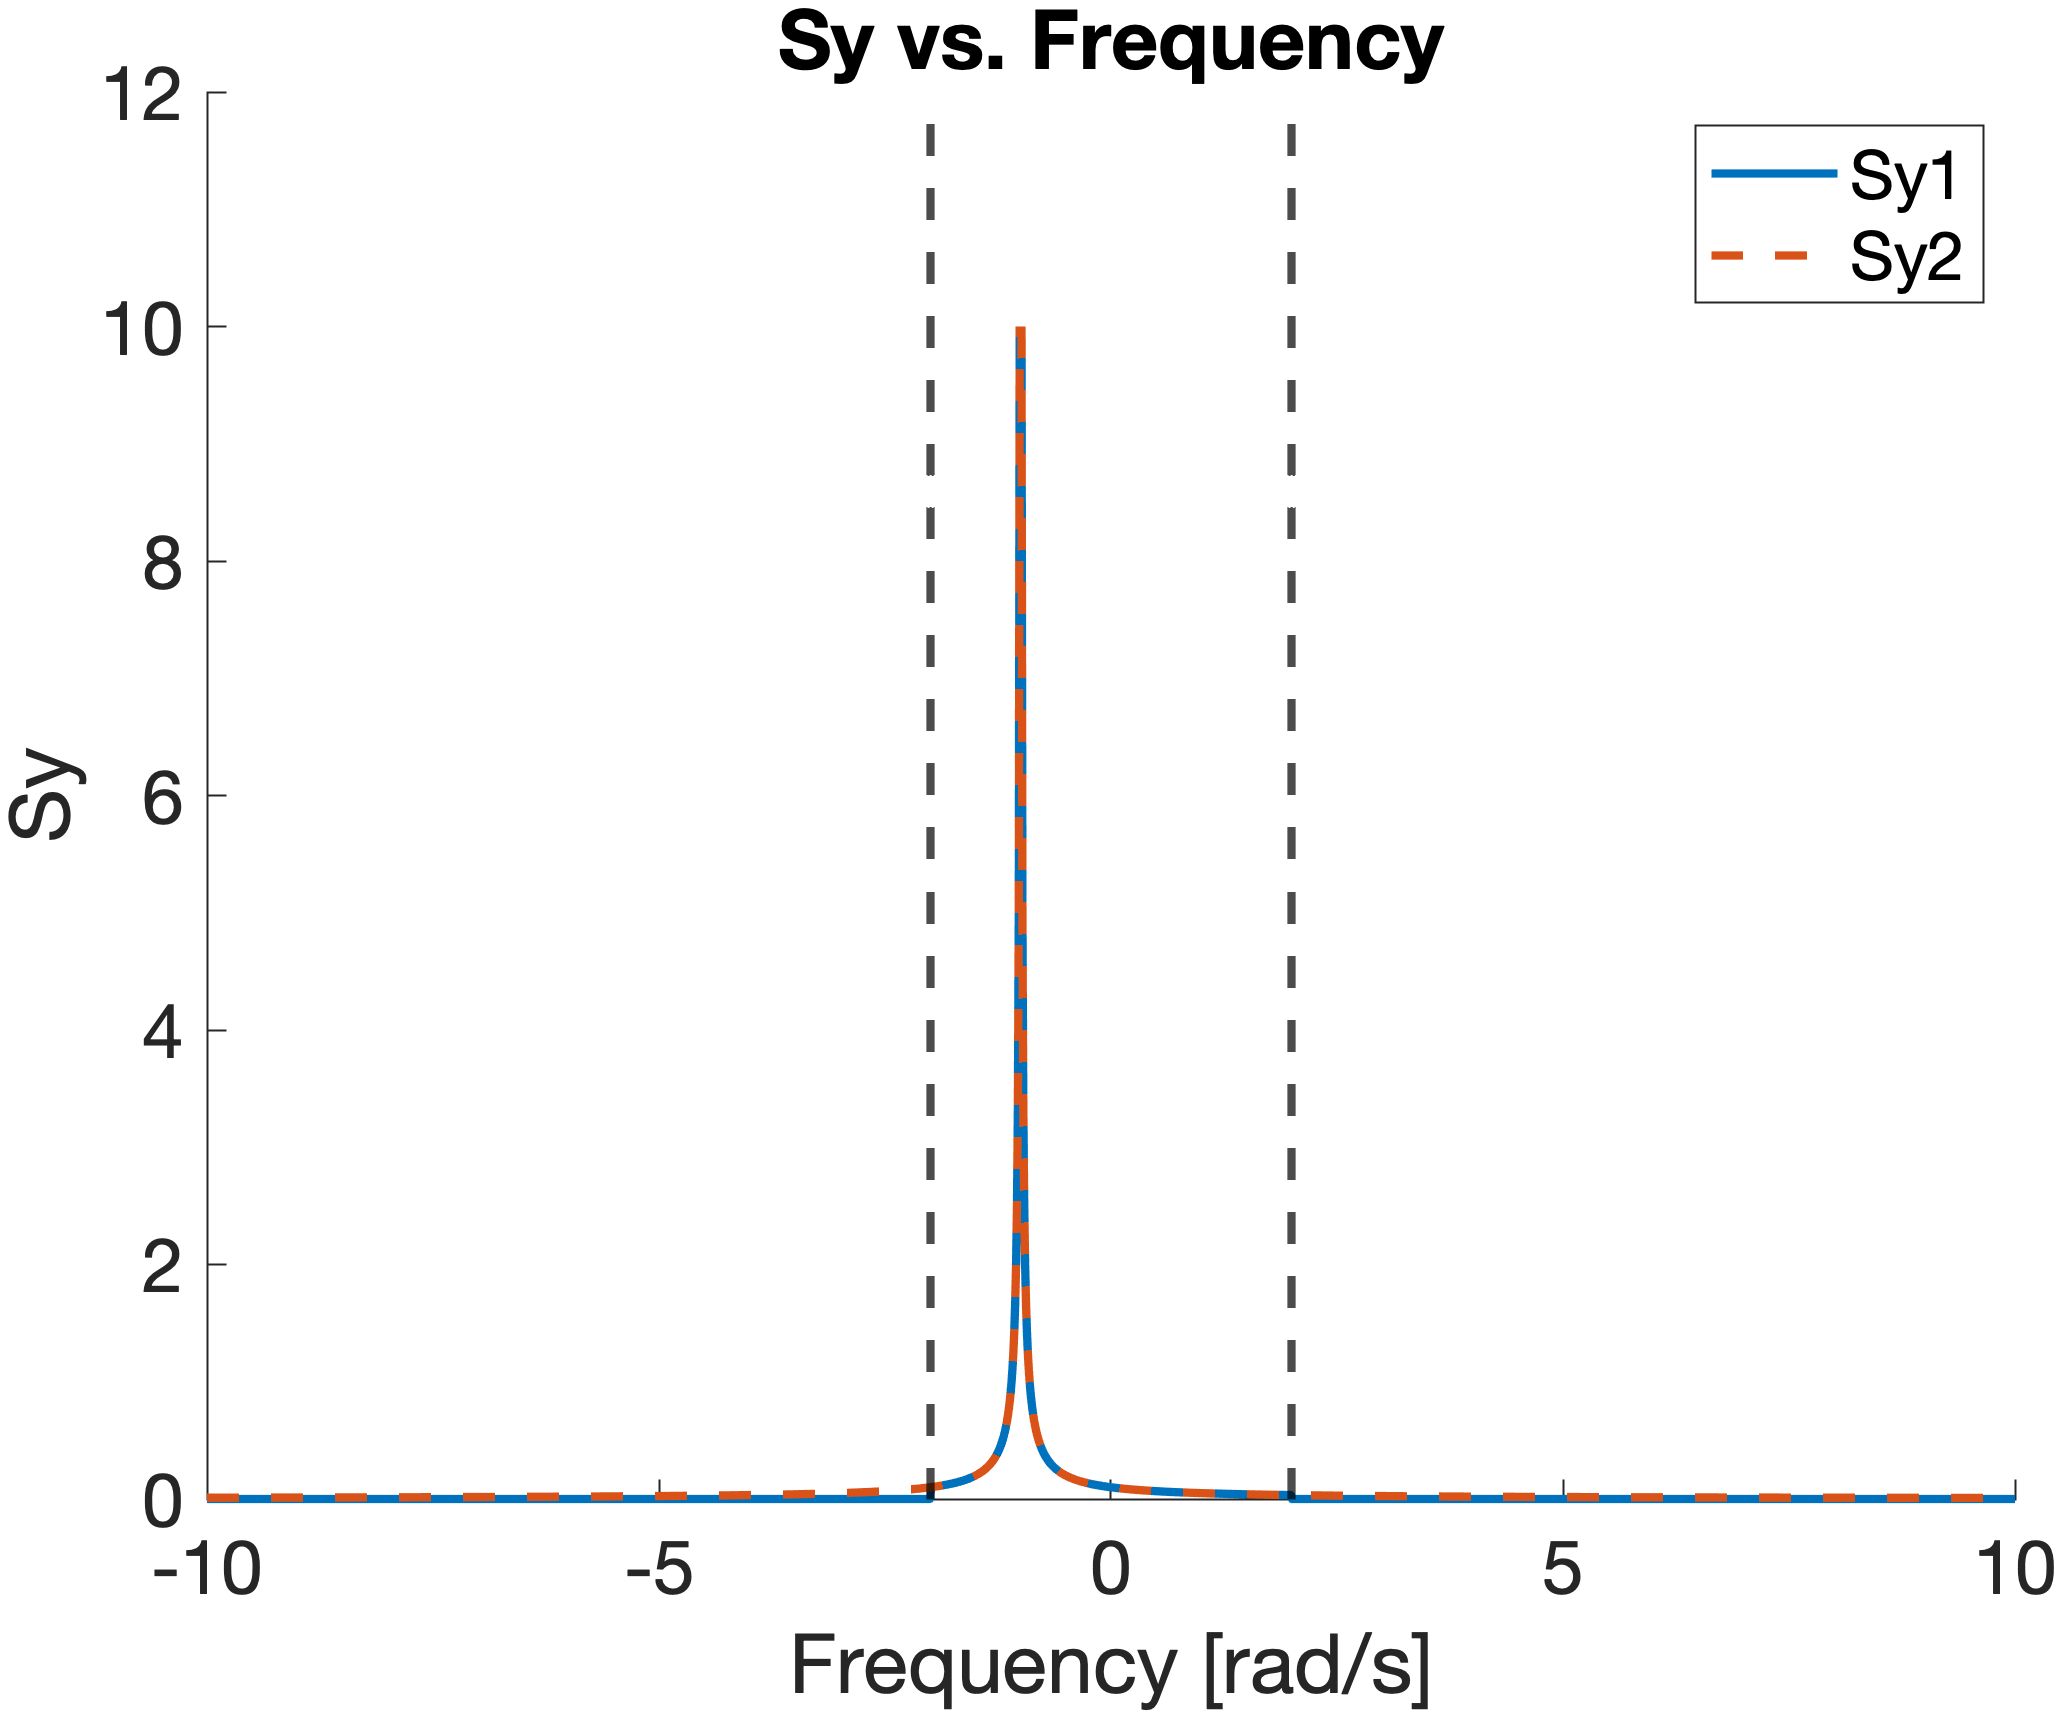
\includegraphics[width=0.75\linewidth]{../figures/p5_sy.png}\label{fig:p5_sy}
    \caption{Sy}
\end{figure}

\subsection*{Part C}
Determine $\left[y^2\right]$ for the two cases.
\subsection*{Solution}
The equation for $y$ is as follows:
\begin{equation}
    y = G(s)w = \frac{w}{T_w s+1}
\end{equation}
where $w$ is white noise.  Given this, the expectation of $y^2$ is calculated as follows:
\begin{gather*}
    E\left[y^2\right] = E\left[(\frac{w}{T_w s+1})(\frac{w}{T_w s+1})\right] \\
    E\left[y^2\right] = E\left[\frac{w^2}{T_w^2 s^2 + 2T_w s + 1}\right] \\
    E\left[y^2\right] = \frac{1}{T_w^2 s^2 + 2T_w s + 1}E\left[w^2\right] \\
    E\left[y^2\right] = \frac{\sigma_w^2}{T_w^2 s^2 + 2T_w s + 1}
    \sigma_y^2 = \frac{\sigma_w^2}{T_w^2 s^2 + 2T_w s + 1}
\end{gather*}
This is true due to the fact that $w$ is zero-mean.

\subsection*{Part D}
Use these results to justify the following statement:
\t If the input spectrum is flat considerably beyond the system bandwidth, there is little error introduced by assuming that the input spectrum is flat out to infinity.
\subsection*{Solution}
Clearly from the above results the difference in bandlimited white noise, and pure, full-spectrum white noise is negligible.  So the above assumption is valid.

\section*{Appendix A: MATLAB Code}

\lstinputlisting[
frame=single,
numbers=left,
style=Matlab-bw
]{../HW2.m}

\end{document}